\chapter{Methods}
%--------------------------------------------------
% GOVERNING EQUATIONS
%--------------------------------------------------
In this chapter we present the physical and mathematical model. The governing equations for this problem are the weakly compressible Stokes flow equations for modeling the viscous flow and the heat transfer equation for computing the time dependent thermal evolution of the system.%Explain a bit each of the subsections


\section{Governing equations}
\subsection{Flow equations}
Stokes flow, also known as creeping flow, describes the motion of viscous, incompressible fluids at very low Reynolds numbers, where inertial forces are negligible compared to viscous forces. Under this regime, the flow is governed by a simplified form of the Navier–Stokes equations, where the inertial terms are omitted. The governing equations consist of the and the conservation of mass, which reduces to the incompressibility condition, and the conservation of momentum, expressed as a balance between the pressure gradient and the viscous forces.
This is vastly assumed to be a proper approximation for solving magmatic flows that imply large time scales, as mantle and magma chamber convection (include citations here). Whereas the Navier-Stokes equations are used to describe short-term phenomena, such as conduit flow or eruptive processes, the steady Stokes flow is a necessary assumption for us, since it's numerical requirements are considerably lower due to the time-scale of the processes we simulate. The equations are expressed as follows:

\begin{align}
	\nabla \cdot (\rho \mathbf{v}) &= 0 \quad \text{in } \Omega, \\
	\nabla \cdot (p\boldsymbol{I} - \tau) &= \rho g\quad \text{in } \Omega,
\end{align}

where $p$ is pressure, $\rho$ is density, $v$ is the velocity vector, $g$ is the gravity vector, $\delta_{ij}$  is identity tensor and $\tau$ is stress tensor which depends on viscosity and strain rate:

\begin{equation}
	\boldsymbol{\tau} = \mu \left( \nabla \mathbf{v} + (\nabla \mathbf{v})^\top \right) - \frac{2}{3} \mu (\nabla \cdot \mathbf{v}) \mathbf{I}
\end{equation}

For which $\mu$ is the viscosity of the mixture.
As our model accounts for phase changes within the magma system, such as crystallization and gas exsolution, we need to also account for the density changes. Thus, we include an isothermal compressibility coefficient transforming our incompressible Stokes system into a weakly compressible one. This coefficient is expressed as:

\begin{equation}
	\beta_T = \frac{1}{\rho}\bigg(\frac{\delta\rho}{\delta p}\bigg)_T
\end{equation}

The set of conservation equations assumes that the different phases we can find in the magma (melt, crystals and gaseous phases) are mechanically coupled, they have the same velocity. This is justified in the frame of high viscosity magmas and time scales of the order of years, and not larger. 
Our system of equations can also be written and solved in a fully coupled monolithic way as a single transport system (Hauke and Hughes, 1998; Longo et al., 2012b; Garg et al., 2018a):
\begin{equation}
	\boldsymbol{F^{a}_{i,i}} = \boldsymbol{F^{d}_{i,i}} + \boldsymbol{S}
\end{equation}


where $\boldsymbol{F_{i,i}^{a}}$, $\boldsymbol{F_{i,i}^{d}}$, and $\boldsymbol{S}$ are the advection flux, diffusion flux and source vectors, respectively, and are defined as:

\begin{equation}
	\boldsymbol{F^{a}_{i}} = 
	\begin{bmatrix}
		\rho v_i\\
		p\delta_{ij} 
	\end{bmatrix}, ~~~~~~~~~~~
	\boldsymbol{F^{d}_{i}} = 
	\begin{bmatrix}
		0\\
		\mathbf{\tau}_{ji}
	\end{bmatrix}, ~~~~~~~~~~~
	\boldsymbol{S} =
	\begin{bmatrix}
		0\\
		\rho g_i
	\end{bmatrix}
\end{equation}

Equation (1) can then be re-expressed for any set of independent variables $\boldsymbol{Y} = [p,\mathbf{v}]$ as follows:


\begin{equation}
	\boldsymbol{A_iY_{,i}} = (\boldsymbol{K_{ij}Y_{,j})_{,i} + S}
\end{equation}


In this equation, $\boldsymbol{A_i = F^{a}_{i,Y}}$ is the $i^{th}$ Euler Jacobian matrix and $\boldsymbol{K = [K_{ij}]}$ is the diffusivity matrix with $\boldsymbol{K_{ij}Y_{,j} = F^{d}_{i}}$.

\subsection{Heat transfer}
In our magma simulations, heat transfer is simulated both inside and outside of the magma domain, although with different approaches. First we solve the heat convection inside the magma domain, as velocity is expected to play an important role on the transport of heat. Then, we couple the boundary of the magma domain with the host rock, trough which the heat will be transferred.

\subsubsection{Magma domain}
Although the fluid motion equations are solved in a fully coupled way as it has been just mentioned, the heat transfer equation needs to be time dependent or transient, since, as opposed to the Stokes assumption, temperature evolves largely with time, as the main process that we are simulating, and the mechanism that controls the evolution of the magma chamber is cooling. The heat transfer equation solved includes advection and diffusion terms, and can be written as follows:

\begin{equation}
	\rho c_p \left(\underbrace{\frac{\partial T}{\partial t}}_{\text{Transient term}} + \underbrace{\mathbf{v} \cdot \nabla T }_{\text{Convection term}}\right) = \underbrace{\nabla \cdot (k \nabla T)}_{\text{Conduction term}} + \underbrace{\mathbf{S}}_{\text{Source term}}
\end{equation}

% \begin{equation}
	% \rho c_p \left( \frac{\partial T}{\partial t} + \mathbf{v} \cdot \nabla T \right) = \nabla \cdot (k \nabla T) + \sum_{i}^{n} \rho_i qL_i \frac{\partial \phi_i}{\partial t}
	% \end{equation}

where $c_p$ is the specific heat capacity, $T$ is the temperature, $\kappa$ is the thermal conductivity and $S$ is any source of sink of heat. Thermodynamical properties of the fluids can be set as fixed or, as they are computed for magma simulations, they can be set as a function of pressure, temperature and composition of the phases. This will be further explained in section XX.

\subsubsection{Rock domain}
The heat transferred across the chamber walls into the host rock is computed by calculating the heat flux along the boundary nodes:

\begin{equation}
	\mathbf{q} = -\kappa_m \nabla T_m
\end{equation}

where $\kappa_m$ and $T_m$ the thermal conductivity and the temperature of the magma respectively. Then, the host rock utilizes the heat flux boundary condition to calculate the heat conduction trough the whole domain:

\begin{equation}
	\rho_r c_{p_r} \frac{\partial T_r}{\partial t} = \nabla \cdot \left( \kappa_r \nabla T_r \right)
\end{equation}

where $\rho_r$ is the rock density, $c_{p_r}$ is the rock specific heat capacity, $T_r$ is the rock temperature and $\kappa_r$ is the rock thermal conductivity.

Once the new temperature profile is computed along the rocks, the new boundary temperature is passed back to the magma, for utilizing in the next time step.

\subsection{Numerical scheme}
Solution is obtained within a single time step by individually iterating over the three sets of equations as described in the following steps:

\begin{enumerate}
	\item Solve the mass and momentum conservation equations. Solution is then passed to the magma heat transfer equation.
	\item Solve the fluid heat transfer equation for the given time step $t_n$ with the velocity solution obtained from the previous step in the form of weak coupling (meaning that we do not correct the Stokes solution after computing the temperature of the system).
	\item Compute the heat flux on the boundary nodes and pass it to the host rock.
	\item From the heat flux obtained from the magma, compute the new temperature distribution inside the host rock and return the boundary temperature to the magma domain to be used on the following time step.
	\item Print the complete solution for the currently solved time step.
\end{enumerate}

The following chart better exemplifies the logic followed within a time step:

\hspace*{-2cm}
\begin{tikzpicture}[node distance=2cm]
	%\node (start) [startstop] {Start};
	\node (step1) [process, xshift=-2cm] {Solve Stokes equations (mass and momentum)};
	\node (decision1) [decision, right of=step1, xshift=2.90cm] {Solution found?};
	\node (step2) [process, right of=decision1, xshift=2.9cm] {Solve temperature equation};
	\node (decision2) [decision, below of=step2, yshift=-1.5cm] {Solution found?};
	\node (step3) [process, left of=decision2, xshift=-2.9cm] {Heat flux from magma to host rock};
	\node (step4) [process, left of=step3, xshift=-3cm] {Solve heat conduction in the rock};
	\node (decision3) [decision, below, below of=step4, yshift=-1.5cm] {Solution found?};
	\node (step5) [process, right of=decision3, xshift=2.9cm] {Set temperature at the interface for next time step};
	\node (stop) [startstop, right of=step5, xshift=2.9cm] {Assemble and print solution for current time step};
	
	\draw [arrow] (step1) -- (decision1);
	\draw [arrow] (decision1) -- (step2) node[midway, above] {Yes};
	\draw [arrow] (decision1.north) to[bend left=-45] node[midway, above] {No} (step1.north);
	\draw [arrow] (step2) -- (decision2);
	\draw [arrow] (decision2) -- (step3) node[midway, above] {Yes};
	\draw [arrow] (decision2.east) to[bend left=-45] node[midway, right] {No} (step2.east);
	\draw [arrow] (step3) -- (step4);
	\draw [arrow] (step4) -- (decision3);
	\draw [arrow] (decision3) -- (step5) node[midway, above] {Yes};
	\draw [arrow] (decision3.west) to[bend left=45] node[midway, left] {No} (step4.west);
	\draw [arrow] (step5) -- (stop);
	% \draw[dashed, red] (current bounding box.south west) rectangle (current bounding box.north east);
\end{tikzpicture}


%--------------------------------------------------
% BENCHMARKS
%--------------------------------------------------
\section{Benchmarking examples}
A number of benchmarking exercises have been made in order to test the accuracy and consistency of the new solver. We show two benchmark exercises for the non-thermally coupled Stokes flow and other four for the complete, thermally coupled solver: SolCx and SolKz from \cite{durez2011}, 2D convection cases 1c, 2a and 3 from \cite{blankenbach1989benchmark}, and 2D cylindrical shell benchmark from ASPECT (\cite{heister:etal:2017,kronbichler:etal:2012,aspect-doi-v2.5.0,aspectmanual}), described as taken from Davies et al case 1.1 BA-Ra104-Iso-ZS (paper yet to be published).

\subsection{SolCx and SolKz}
This two benchmarks test the accuracy of the stand-alone Stokes equations with varying viscosity. The domain is in both cases a square box ($l/h = 1$) with all boundaries set to be free slip.
In the case of SolCx, fluid flow is driven by a sinusoidal force:
\begin{equation} 
	F = (0,-sin(\pi y)cos(\pi x))
\end{equation}
and a sharp viscosity jump set as follows:
\begin{equation}
	\eta (x) =
	\begin{cases} 
		1, & \text{if } 0 \leq x \leq 0.5 \\
		10^6, & \text{if } 0.5 < 0 \leq 1 Ma
	\end{cases}
\end{equation}
For the SolKz case, the driving force should be expressed as:
\begin{equation} 
	F = (0,-sin(2y)cos(3\pi x))
\end{equation}
while the viscosity distribution is defined as:
\begin{equation}
	\eta(y)=exp(2By)
\end{equation}
Results for both benchmarks are depicted in figure \ref{fig:sols}, matching perfectly the benchmark results described in the reference paper, hence assessing the Stokes solver accuracy.
\begin{figure}
	\centering
	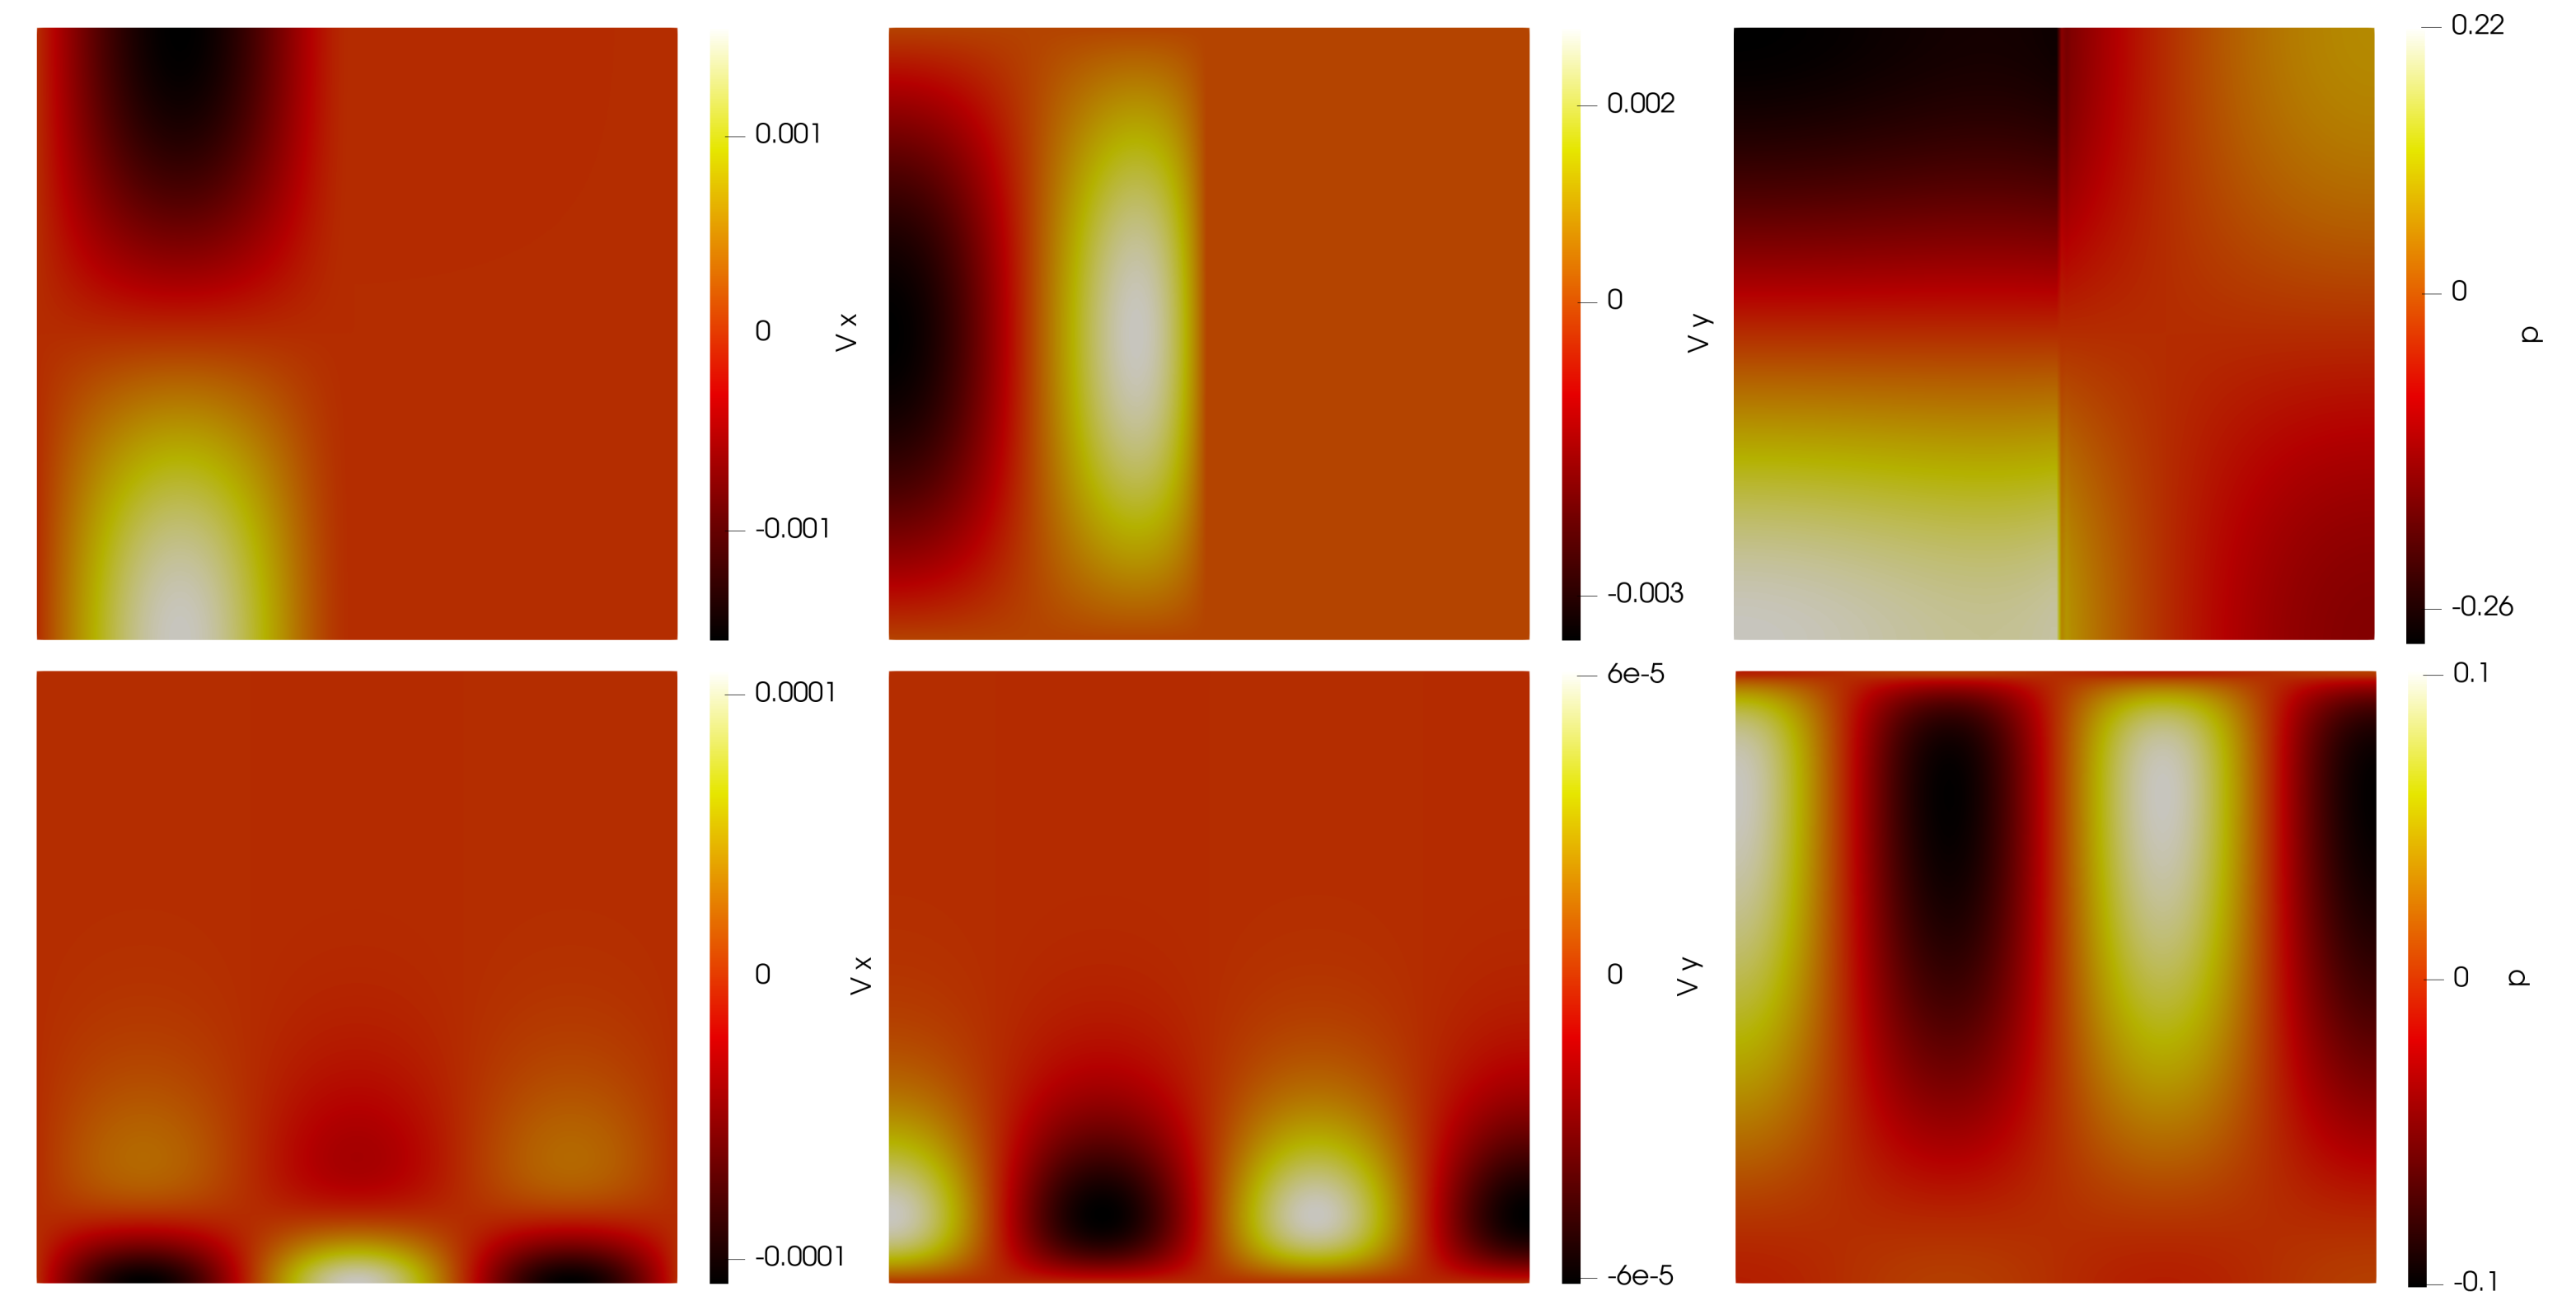
\includegraphics[width=1\linewidth]{img/chapter2/benchmarks/sols.png}
	\put(-442,100){SolKz}
	\put(-442,200){SolCx}
	\caption{Horizontal and vertical velocity fields as well as and pressure distribution for SolCx benchmark on top, and SolKz benchmark on the bottom of the figure}
	\label{fig:sols}
\end{figure}

\subsection{2D convection 1c}
This benchmark is described as steady convection with constant properties, including constant viscosity. Domain is a square box ($l/h = 1$) and the temperature is fixed to zero on top and to $\Delta T$ on bottom. There are no internal heat sources. No normal-velocity flux on the side boundaries (reflective symmetry conditions) and free slip condition (zero shear stress) on all boundaries. The Rayleigh number is
\begin{equation}
	Ra = \frac{\alpha g \delta T h^3}{\kappa \mu}
\end{equation}
and for this case it is set to have a value of $10^6$.
This benchmark requires calculating the Nusselt number as in:

\begin{equation}
	Nu = -\frac{\int_{0}^{1}\delta_zT(x,z=h)dx}{\int_{0}^{1}T(x,z=0)dx}
\end{equation}
the root-mean-square (rms) velocity:

\begin{equation}
	v_{rms} = \frac{h}{\kappa} \bigg[\frac{1}{hl}\int_{0}^{l}\int_{0}^{h}(u^2+w^2)dzdx\bigg]^{\frac{1}{2}}
\end{equation}

and the temperature gradients at the corners:

\begin{equation}
	q = \frac{-h}{\Delta T}\bigg(\frac{\delta T}{\delta z}\bigg)
\end{equation}

All of this three quantities are non-dimensional in this examples. Results are within the benchmark limits, with a Nusselt number of 20.73, a v$_{rms}$ of 849.97, q$_1$ equal to 34.5 and q$_2$ equal to 0.863.  
Figure \ref{fig:convection_1c} shows the temperature distribution at the steady state of the simulation, showing a right-wise convective pattern.


\subsection{2D convection 2a}
In this case, non dimensional viscosity is temperature and depth dependent following this equations:
\begin{equation}
	\mu = \mu_0 exp\bigg[-\frac{bT}{\Delta T} + \frac{c(1-z)}{h}\bigg]
\end{equation}
with $b = ln(1000)$ and $c = 0$ and $\mu_0$ is 1 in its dimensionless form. Boundary conditions for this case are the same as for the previous one and Rayleigh number has a value of $10^4$. Requirements for this example are the same as for the previous one (case 1c).
The results for this quantities are: Nu equal to 10.29, v$_rms$ equal to 499.74 and q$_1$ and q$_2$ equal to 18.04 and 1.01 respectively. 
Figure \ref{fig:convection_2a} shows temperature and temperature contours distributions and velocity and with streamlines once steady state is achieved. 

\subsection{2D convection 3}
This time-dependent case of convection has constant viscosity and internal heating. The domain changes to an aspect ratio of $l/h = 1.5$. Side boundaries again have reflective symmetry conditions. No-slip conditions on top and bottom. Temperature at the top is zero, while at the bottom of the domain, the heat flux is zero.


\subsection{2D cylindrical shell}
This case is described as a 2D non-dimensional spherical earth with an outer radius on 1.22 and an inner radius of 2.22. Temperature is 1 in the internal boundary (inner radius) and 0 in the outer as an initial condition. Boussinesq approximation is assumed, and non-slip boundary conditions. Rayleigh number is $10^4$ and the initial temperature distribution follows a spherical harmonic of degree 0 and order 4.
The simulation should arrive to an steady state stage in which four convective cells have formed, staged that is successfully reached, as seen in figure \ref{fig:cylindrical_shell}.

\begin{figure}
	\centering
	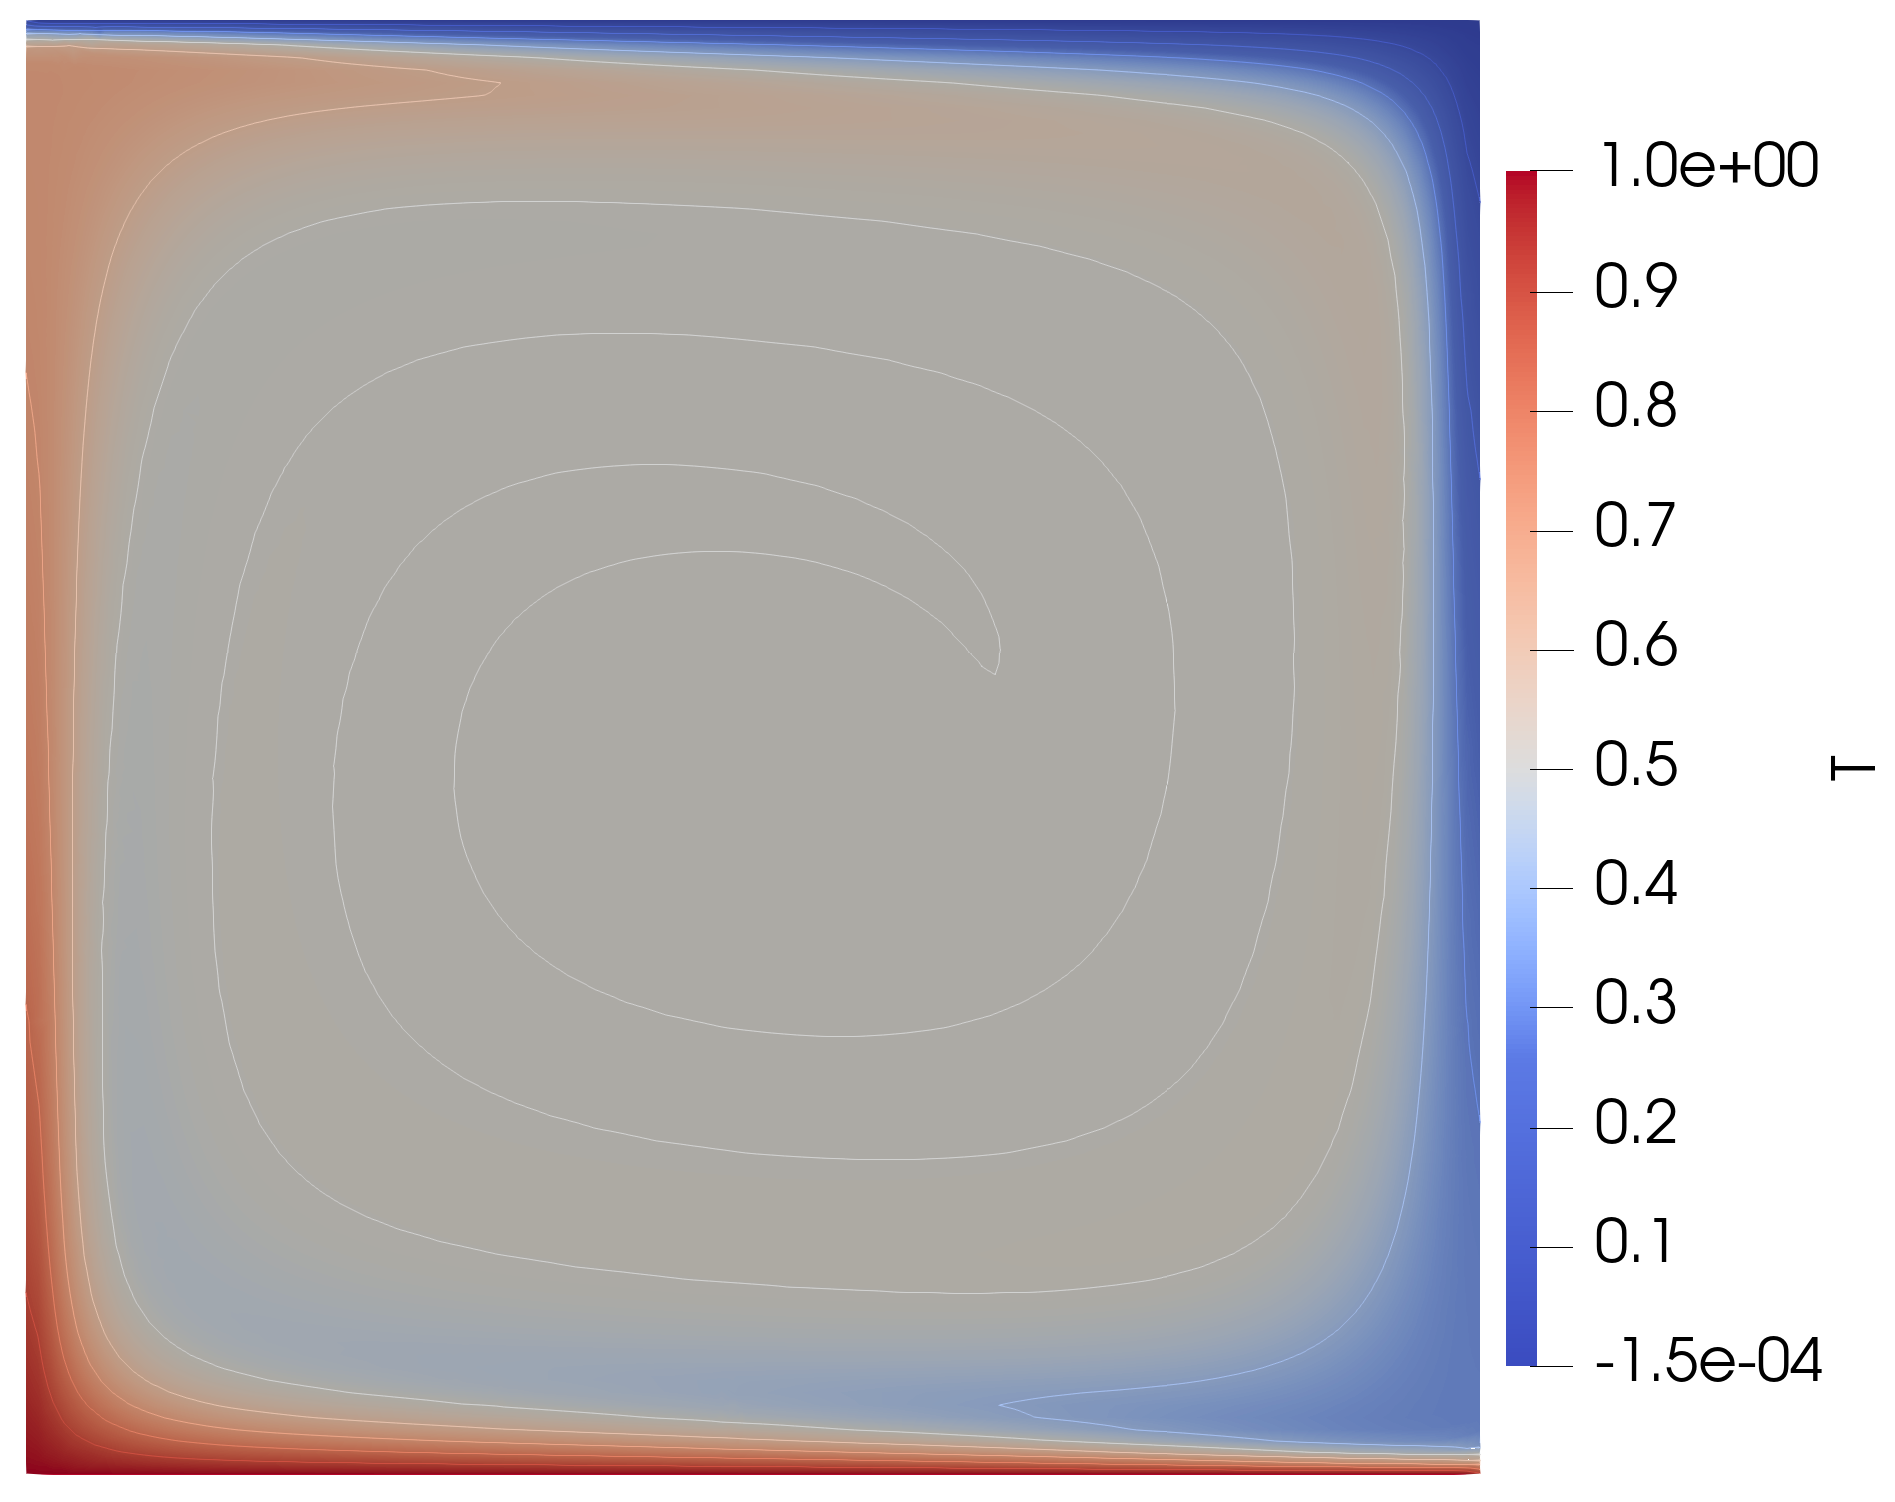
\includegraphics[width=0.75\linewidth]{img/chapter2/benchmarks/contours.png}
	\caption{Temperature field for the 2D convection 1c benchmark once it has reached the final steady state stage}
	\label{fig:convection_1c}
\end{figure}


\begin{figure}
	\centering
	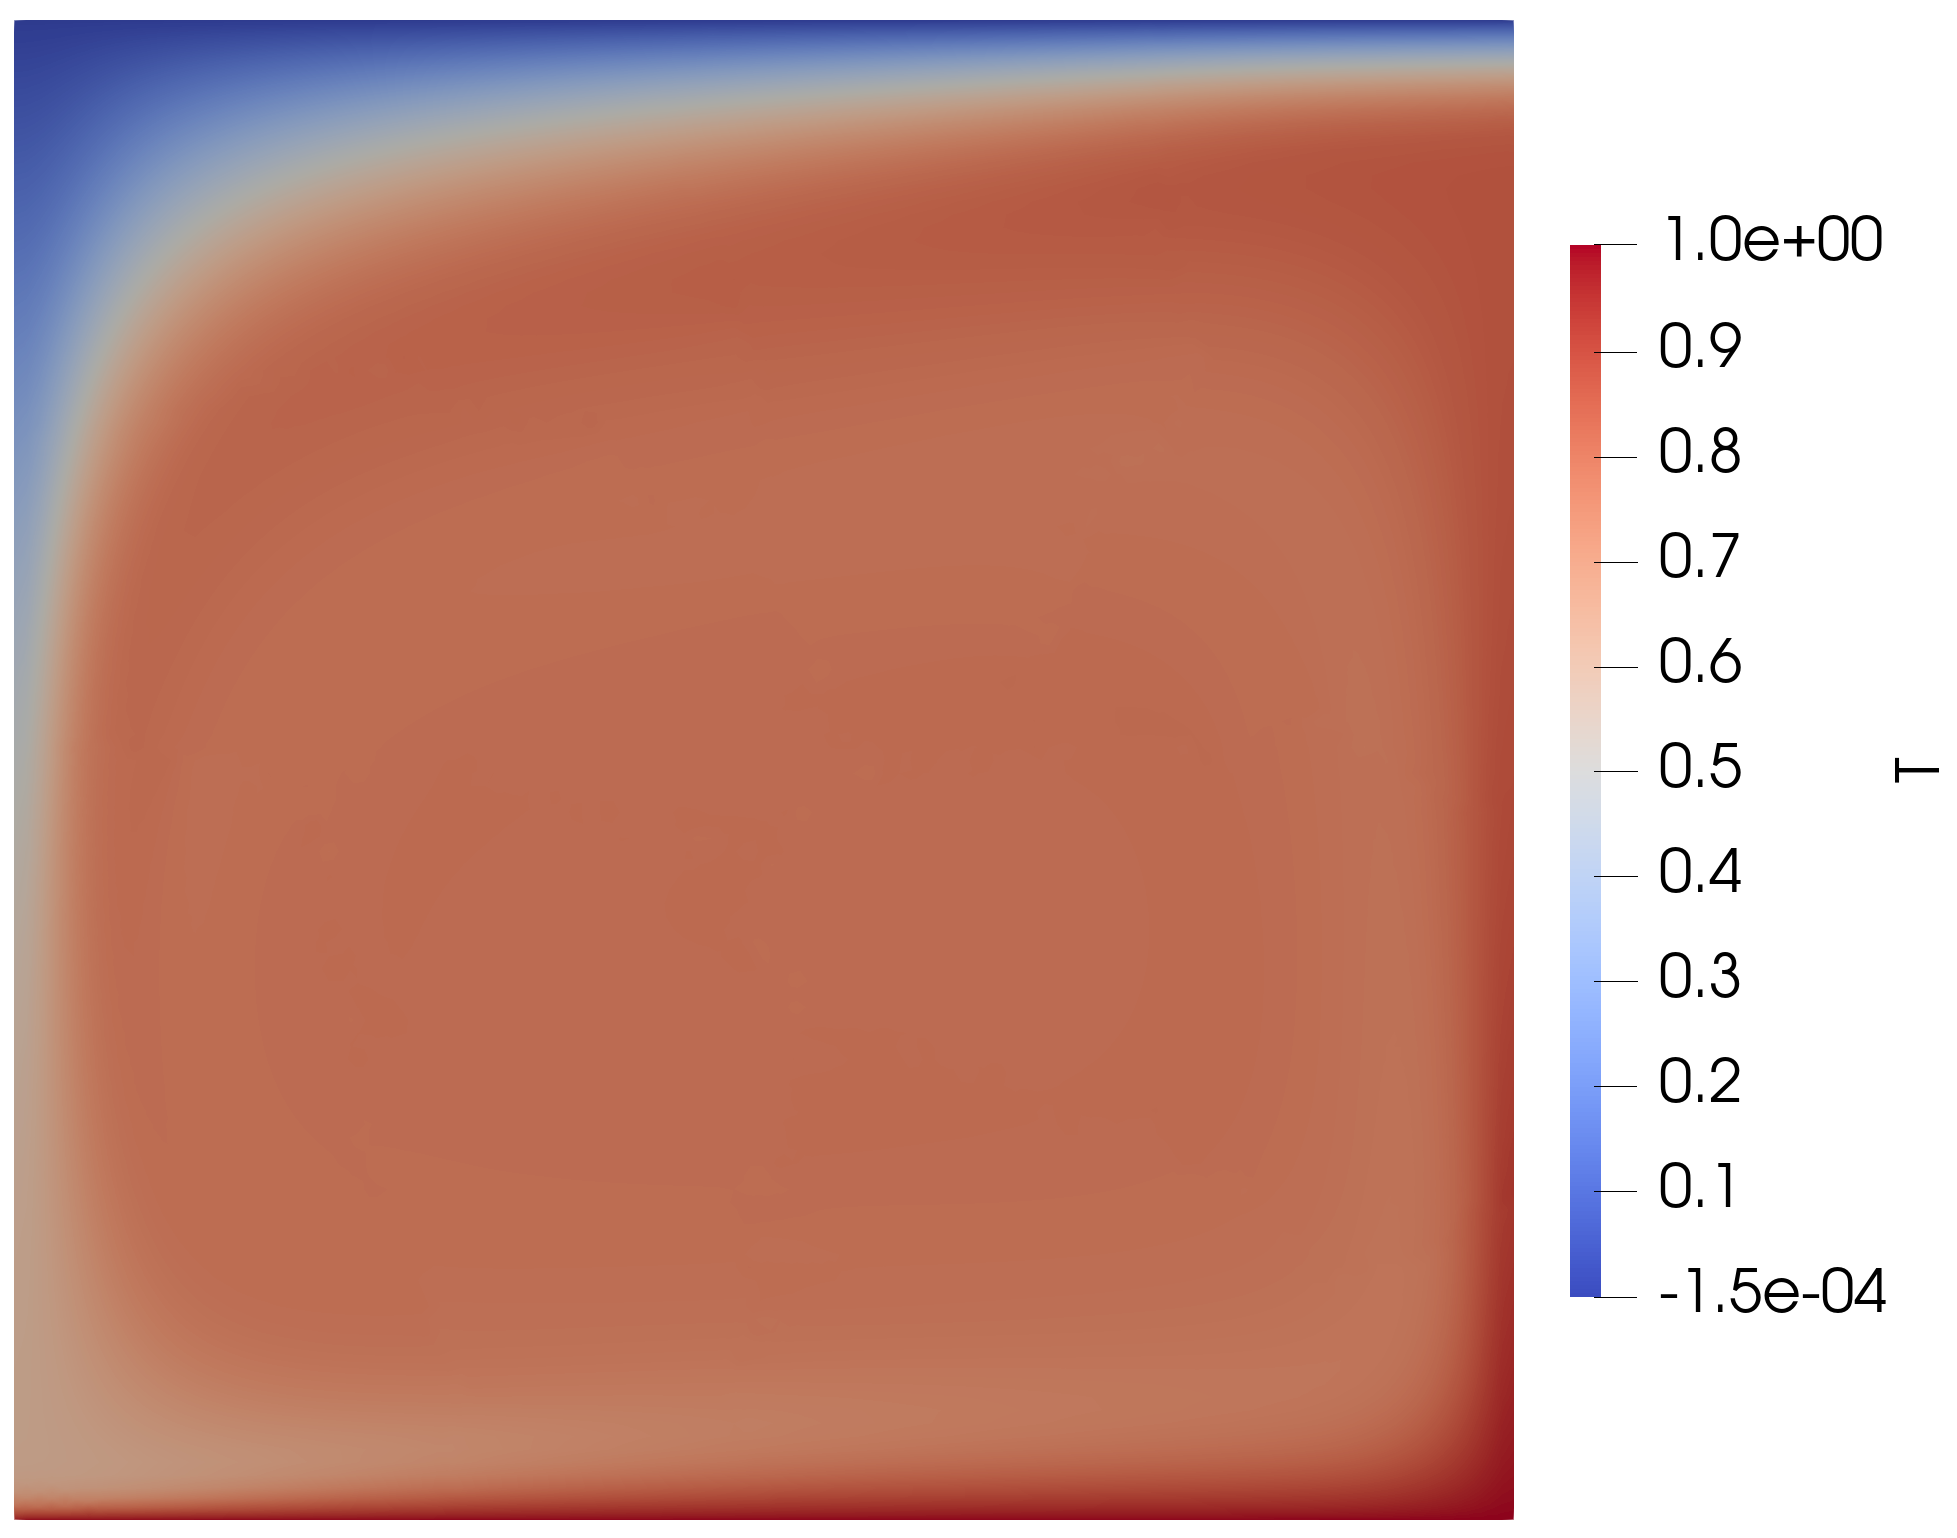
\includegraphics[width=0.75\linewidth]{img/chapter2/benchmarks/temp.png}
	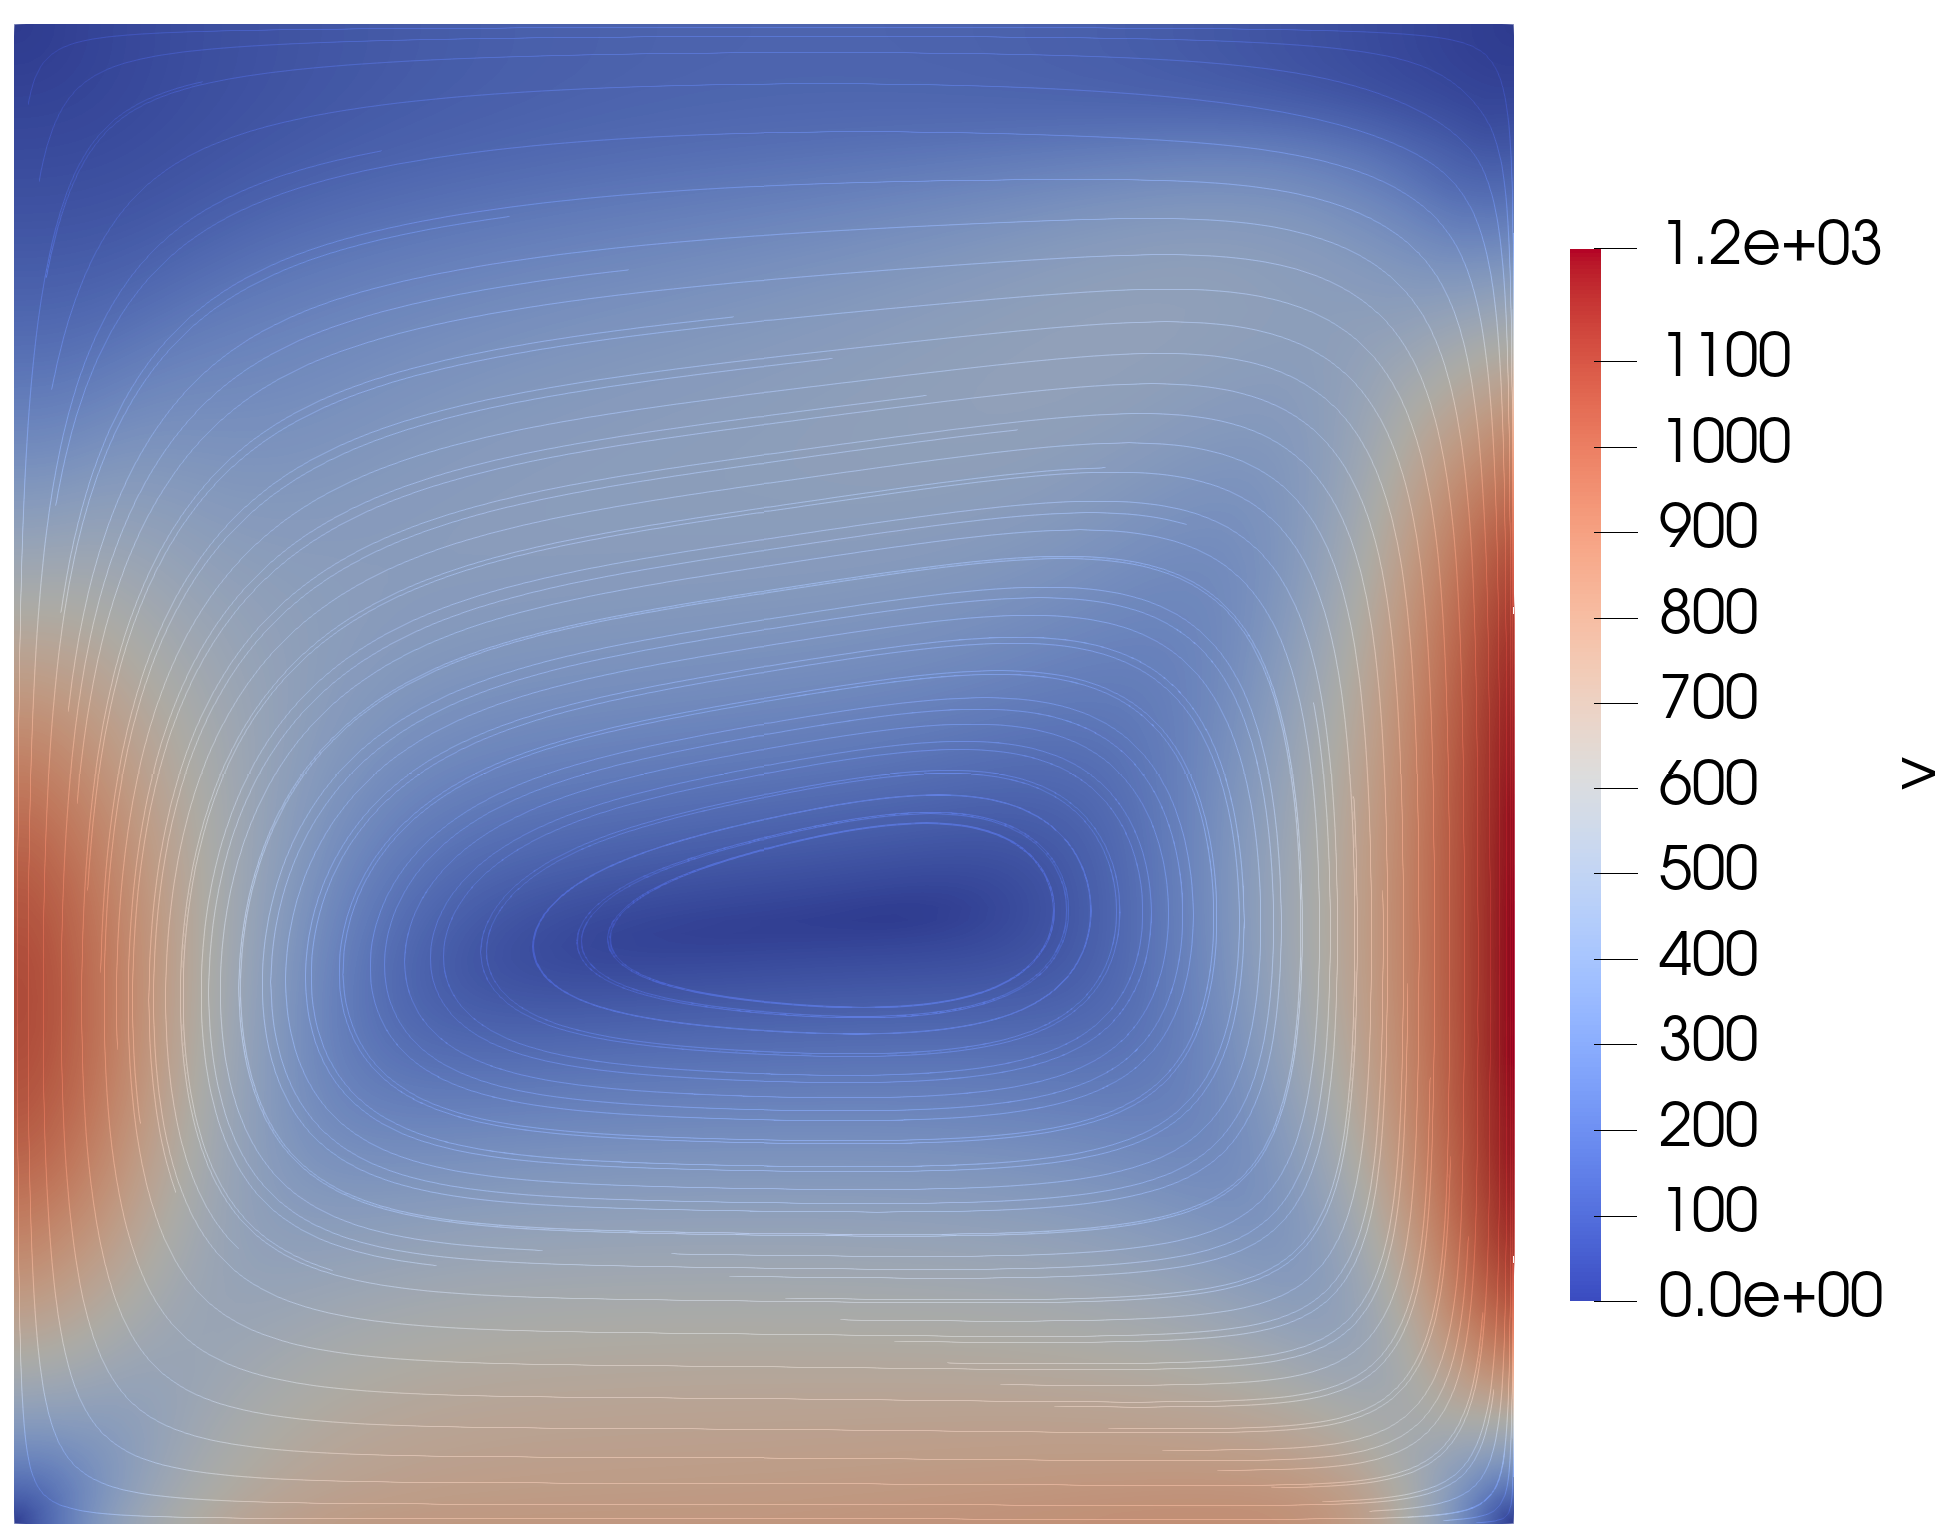
\includegraphics[width=0.75\linewidth]{img/chapter2/benchmarks/streamlines.png}
	\caption{Temperature field for the 2D convection 1c benchmark once it has reached the final steady state stage}
	\label{fig:convection_2a}
\end{figure}

\begin{figure}
	\centering
	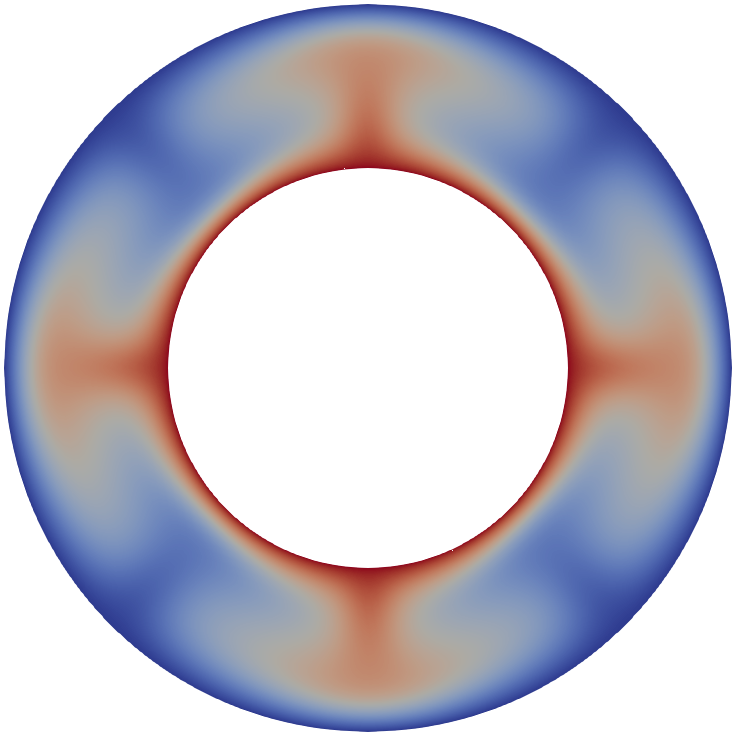
\includegraphics[width=0.75\linewidth]{img/chapter2/benchmarks/t_1.png}
	\caption{Temperature field for the 2D cylindrical benchmark once it has reached the final steady state stage}
	\label{fig:cylindrical_shell}
\end{figure}


\subsection{OUR OWN BENCHMARK}
% Develop a simple crystallization and exsolution temperature equations, just normal relationships with T (and P?) 
Due to the significant lack of benchmarking exercises for the thermally coupled stokes flow under magmatic conditions, we propose a benchmark simulation. A simple setup is presented: a rectangular magma chamber 1250 meters long and 500 meters high, with an outer 500 meters rectangle that is set to be the host rock. Initial pressure of the magma is 50 MPa at the top, evolving towards the bottom according to  , while the initial temperature is 900°C. Initial temperature of the surrounding rocks is 350°C. No-slip condition is applied to all boundaries of the magma domain.  
Crystallization and exsolution are defined as simple temperature dependent exponential functions as follows the:

% \begin{equation}    
	% \begin{array}{cc}
		%     \phi_{cryst}(T) =
		%     \begin{cases} 
			%     0.1, & T \leq 700 \\
			%     0.1* \left(\frac{900 - T}{200} \right)^2, & 700 < T \leq 900 \\
			%     0, & T > 900
			%     \end{cases}
		%     & \ \ \ \ \ \ \
		%     \phi_{gas}(T) =
		%     \begin{cases} 
			%     1.0, & T \leq 700 \\
			%     \left(\frac{850 - T}{200} \right)^2, & 700 < T \leq 850 \\
			%     0, & T > 850
			%     \end{cases}
		% \end{array}
	% \end{equation}

\begin{equation}   
	\phi_{cryst}(T) =
	\begin{cases} 
		1, & T \leq 700 \\
		0.1* \left(\frac{850 - T}{150} \right)^2, & 700 < T \leq 850 \\
		0, & T > 850
	\end{cases}
\end{equation}

\begin{equation}
	\phi_{gas}(T) =
	\begin{cases} 
		0.1, & T \leq 700 \\
		\left(\frac{900 - T}{200} \right)^2, & 700 < T \leq 900 \\
		0, & T > 900
	\end{cases}
\end{equation}

This functions ensure a fully crystallized and exsolved magma at temperatures bellow 700°C and a fully melted magma at temperatures above 900°C, as can be easily appreciated in figure \ref{fig:phi_benchmark}.

\begin{figure}
	\centering
	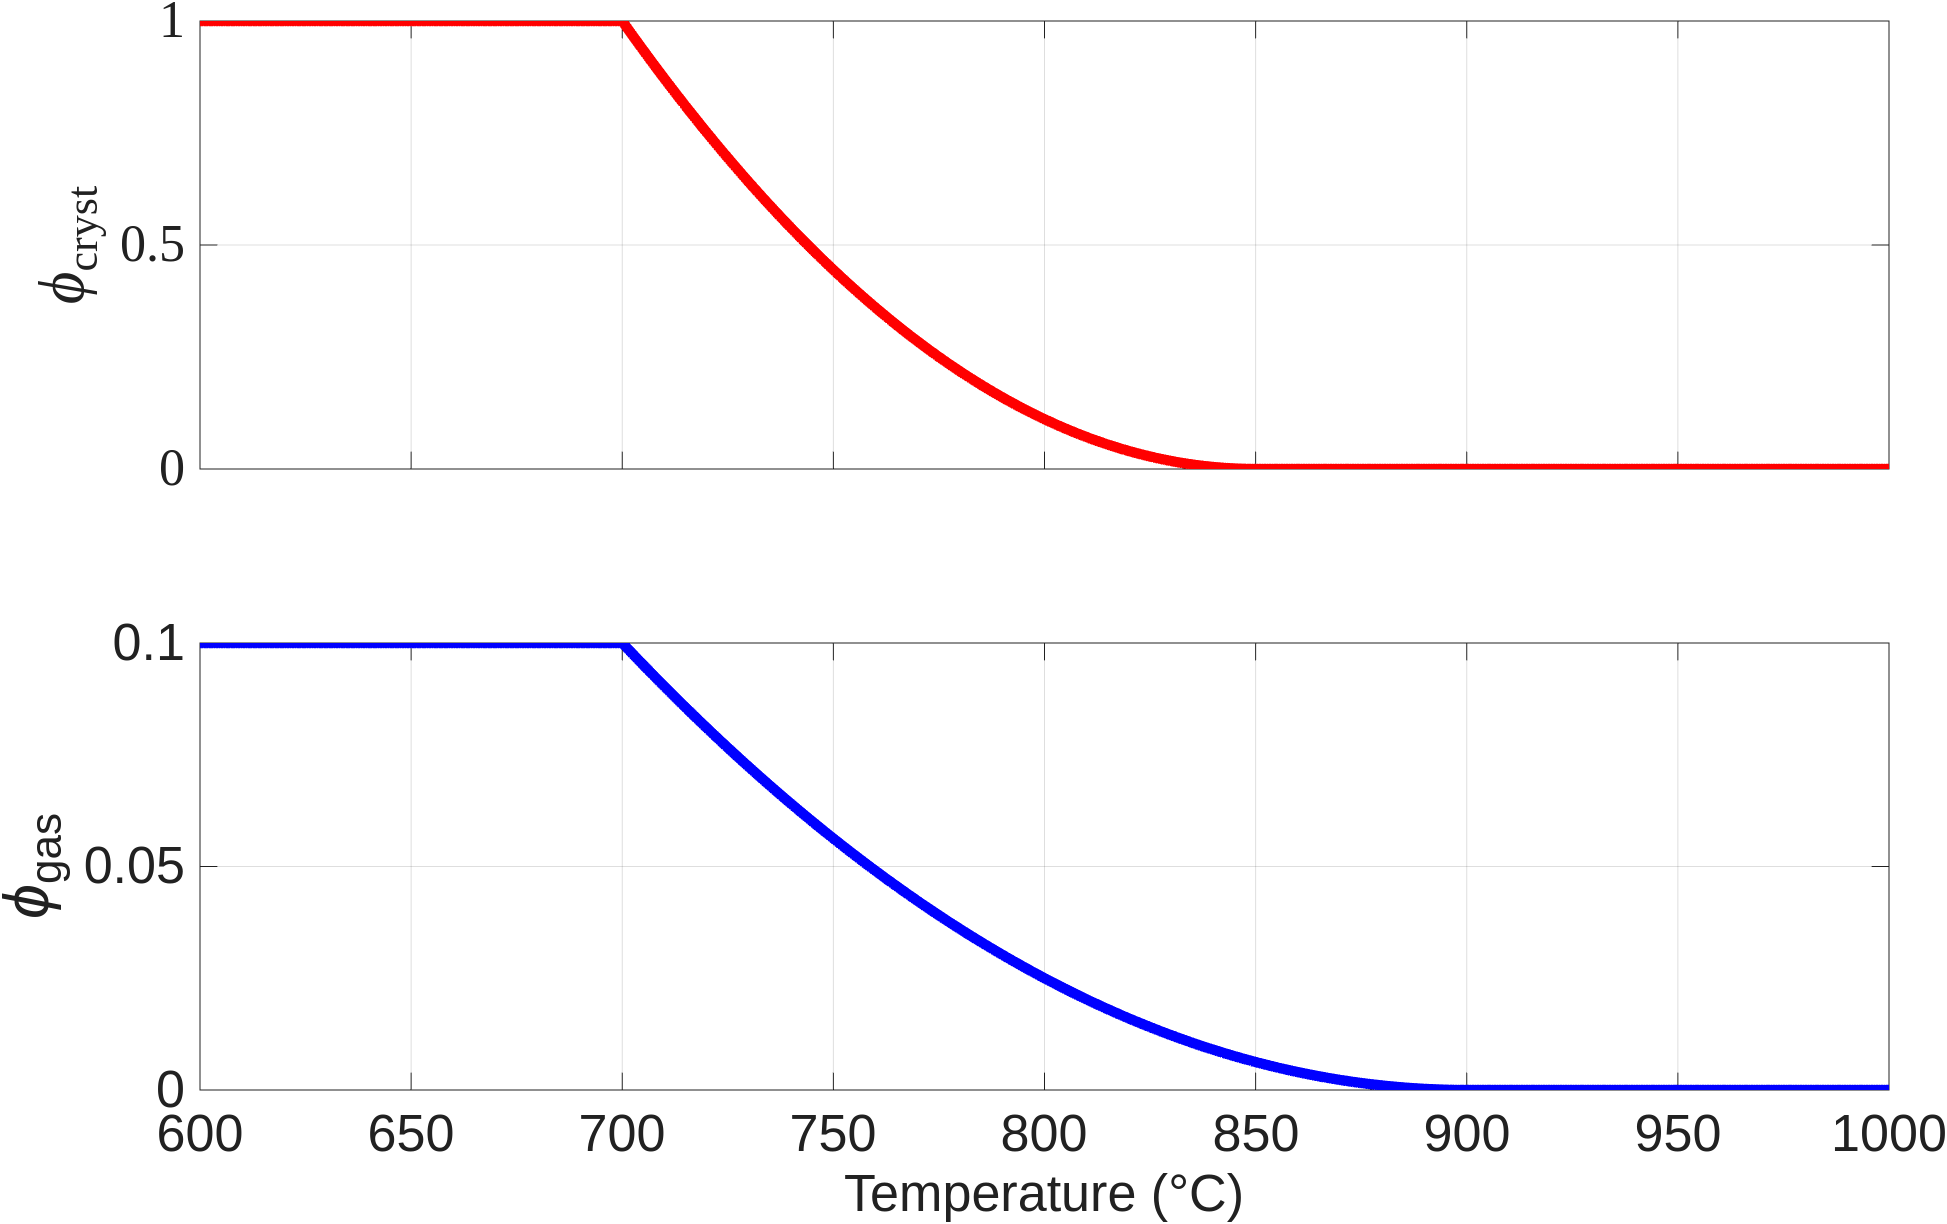
\includegraphics[width=1\linewidth]{img/chapter2/benchmarks/phis.png}
	\caption{Crystal and gas fractions exsolution curves for the proposed benchmark exercise}
	\label{fig:phi_benchmark}
\end{figure}

The properties for each phase are described in the following table:

\begin{table}[H]
	\resizebox{\columnwidth}{!}{%
		\begin{tabular}{|c|c|c|c|c|}
			\hline
			& density($g/m^3$) & thermal conductivity($W/mK$) & specific heat capacity($J/kg°C$) & latent heat($J/kg$)\\ 
			\hline
			Melt & 2400 & 1.0 & 1300 & \\
			\hline
			Crystals & 2600 & 3.0 & 1000 & 200000\\
			\hline
			Gas & 200 & 0.1 & 2000 & -100000\\
			\hline
		\end{tabular}
	}
	\caption{Material properties for the different phases present in the magma, for the proposed benchamr simulation}
	\label{tab:benchmark_props}
\end{table}


\section{Thermomechanical modeling}
\subsection{Magma properties}
Physical properties are fundamental in the understanding of the behavior and evolution of magmas. They determine the velocity at which magmas move, how fast they cool, how they crystallize and even erupt. For instance, density controls buoyancy and has an strong influence on whether a magma will ascent, stall, or sink, directly influencing magma chamber formation. Heat capacity dictates how much energy a magma is able to store and how resistant it is to temperature variations, affecting the longevity and thermal stability of magma bodies. Thermal conductivity regulates how efficiently magmas lose heat to surrounding rocks, shaping the rate of crystallization and the thermal evolution of intrusive systems. Viscosity controls magma mobility, eruption style, and even the formation of crystal mushes. 

Thus, their importance is of the utmost essence, and need to be properly and realistically modeled in order to maximize the resemblance between the simulated results and reality.  As most of the properties are well constrained by diverse models and natural observations, they serve as the link between the computational domain and the natural world. 

In our simulations, the magmatic properties are computed as a bulk quantities, meaning that the three coexisting phases contribute to the total value of a said property proportionally to its abundance within the magmatic system.
\subsubsection{Temperature}
Temperature constitutes one of the, if not the most important variables controlling magma generation, evolution and overall behavior. It determines whether rocks remain solid, partially or fully molten, and it directly influences fundamental properties such as viscosity, density and crystallinity. Higher temperatures promote low viscosity magmas, magmas capable of flowing and convecting. Cooling drives crystallization, increases viscosity, and eventually leads to solidification. Temperature also controls phase equilibria, determining which minerals crystallize at different stages and influencing the chemical differentiation of magma. Additionally, it affects the solubility of volatiles, the rate of diffusion and the kinetics of chemical reactions. In magma chambers, spatial and temporal variations in temperature can create thermal gradients that drive convection, melt segregation, and even reactivation of previously solidified zones. Overall, temperature is not only a measure of thermal energy but a key control on the dynamics, structure, and eruptive behavior of magmatic systems.

In the present study, temperature is both the solution of the heat transfer equations and an input parameter in computing the phase equilibria and magmatic properties. It is of the upmost importance when analizing results
\subsubsection{Pressure}
Pressure is, alongside temperature, a fundamental variable in any magmatic system with a profound effect on the physical, chemical and phase behavior of magma. It strongly controls gas solubility, favoring volatile dissolution at higher pressures, thereby affecting magma viscosity, crystallization temperatures, and eruptive potential. It is also important on determining melting and crystallization paths. As magma ascends toward the surface, decreasing pressure triggers volatile exsolution, bubble growth, and potentially explosive eruptions if gas escape is restricted. Changes in pressure also shift mineral stability fields, influencing which phases crystallize and when, thus shaping the final rock paragenesis. Furthermore, pressure affects magma chamber dynamics by modulating buoyancy, convection, and the potential for magma recharge or chamber collapse.

Pressure is computed as part of the solution of the Stokes equations alongside the velocity. The initial pressure distribution, however, is computed to be a horizontally uniform profile.

\subsubsection{Volatiles}
Volatiles make up for the one of the three possible phases that are found in magmas, alongside melt and crystals. The most abundant one is water ($H_2O$), followed by carbon dioxide ($CO_2$), and, normally in smaller amounts than the first two, sulfur species ($SO_2$ and $H_2S$) and others. These gases have a profound influence in the physical behavior of magmas, as well as in their chemical evolution, and have major importance regarding eruptive dynamics. Gases in magmas can be found dissolved in the fluid phase when pressure is sufficiently high, and exsolved, forming bubbles in the magma. Dissolved volatiles reduce the viscosity and lower the liquidus of the melt, delaying the formation of crystals and enhancing magma mobility. On the contrary, the role of bubbles can either reduce or increase the viscosity of the magma, as will be discussed further below. Bubble formation normally leads to magma overpressure and, ultimately, volcanic eruptions. Also, the amount and type of volatiles have an deep control on weather an eruption es effusive or explosive.

In this work, the partition between the dissolved and exsolved volatiles is done utilizing the equation of state of SOLWCAD (\cite{papale2006}). SOLWCAD is a numerical software initially written in FORTRAN that computes the fully non-ideal and multi-component compositional-dependent saturation surface of $H_2O$ and $CO_2$ in silicate melts over a wide range of pressure and temperature conditions. The software has been rewritten in C++ and implemented within GALES  to allow run-time gas-equilibria computations for any P-T-X inside the magma domain. 

\begin{figure}
	\centering
	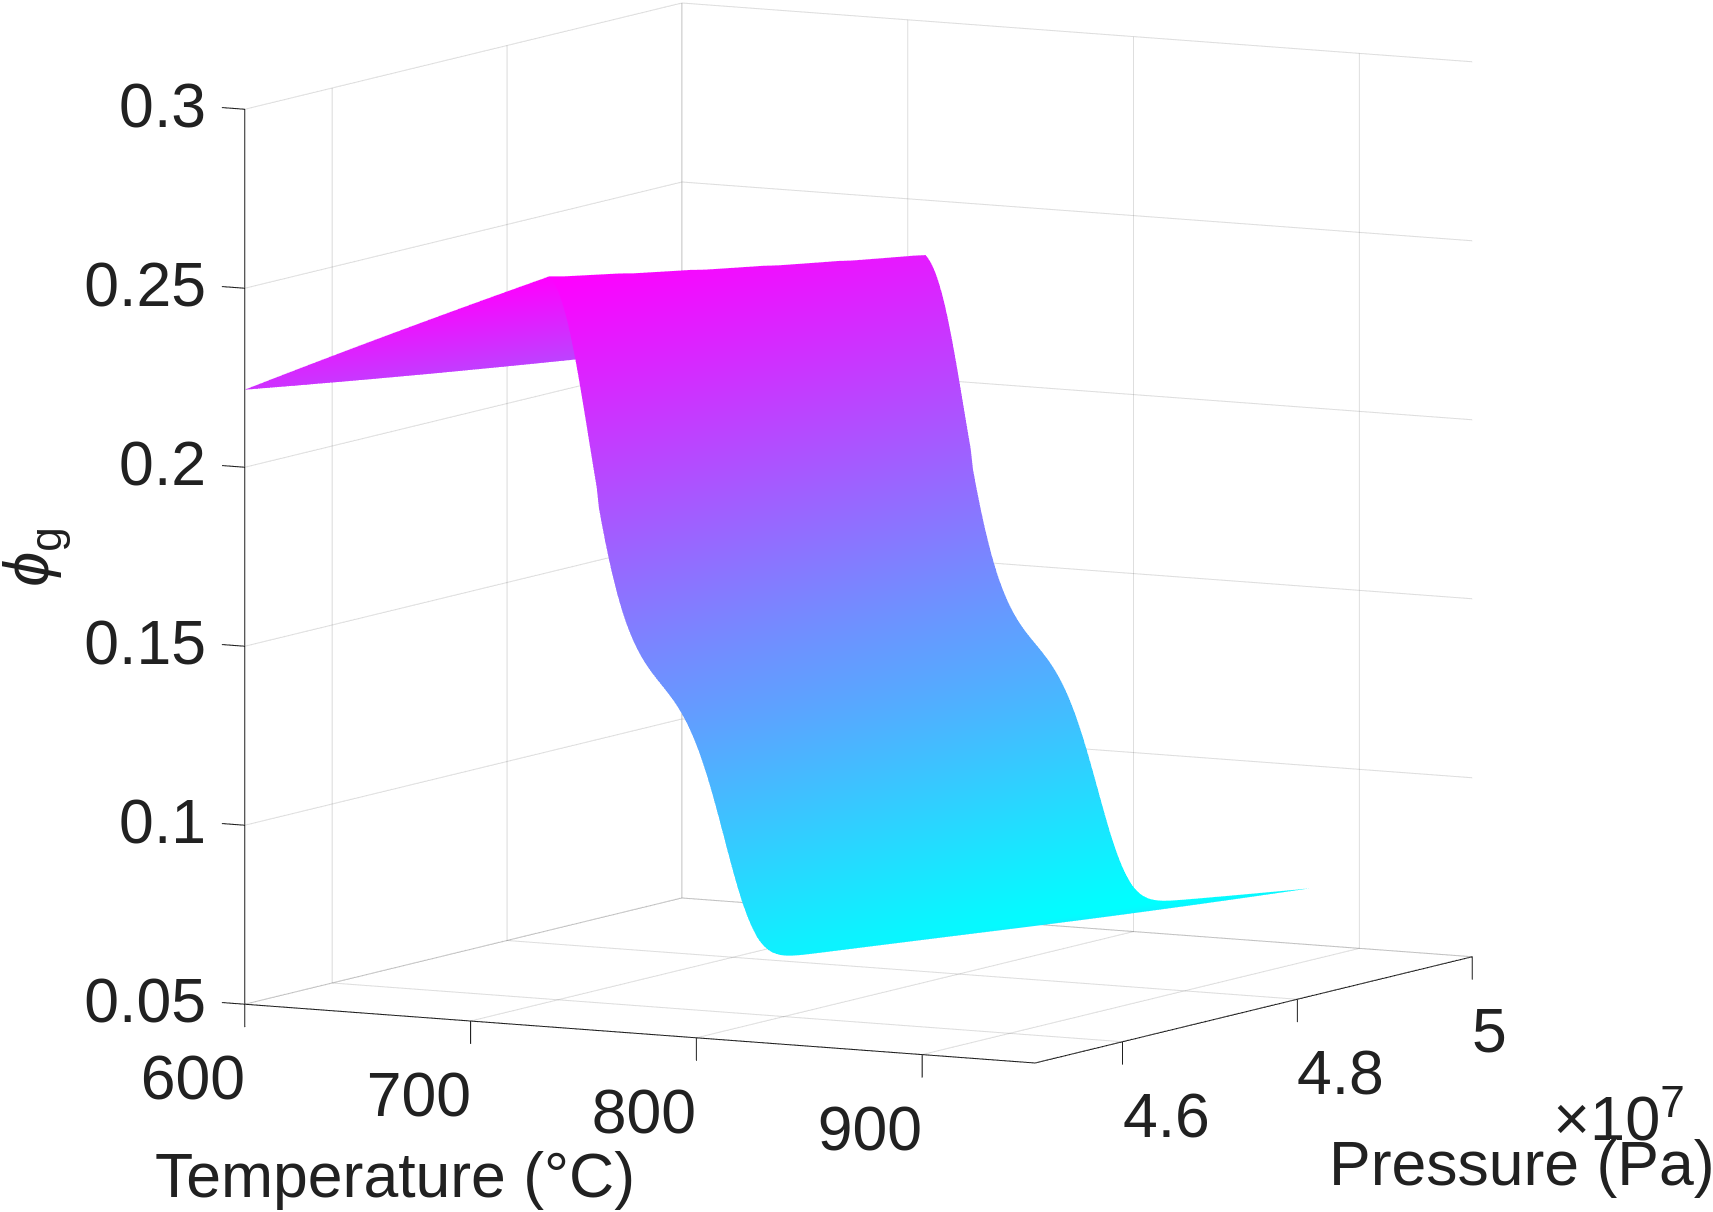
\includegraphics[width=1\linewidth]{img/chapter2/properties/vf_g/vf_g.png}
	\caption{Bulk thermal conductivity modeled for 45 MPa}
	\label{fig:volume_gas}
\end{figure}

\subsubsection{Crystallinity}
Crystallinity is crucial in the understanding of magmas evolution, as it serves as an indicator of its thermal, chemical and mechanical state. As magmas cool, they normally undergo partial crystallization, influencing properties such as viscosity, density and thermal conductivity, but not only, since the impact of crystallinity also extents to the magma dynamics and eruptive potential and style. Magmas with low crystal fraction behave as fluids, capable of mixing and flowing, while high-crystallinity ones (typical more than 50\% crystal fraction) typically form rather immobile crystal mushes. Crystallinity plays a fundamental role in magma differentiation, as melt segregation is normally produced due to crystal accumulation, modifying melt and mineral composition, and leading to the generation of evolved magmas.

Crystal fraction can be computed from a number of numerical models, empirical data calculated from petrological observations or simply by setting a fixed a unique value, typical for isothermal simulations. Within GALES, any of these can be easily implemented. For this work, the relation obtained by \cite{abdullin2024} from laboratory experiments on silicic samples is used. This has the advantage of being numerically efficient, as for us it is just a simple mathematical relation.

\begin{equation}
	\begin{aligned}
		T_i = T_c - 273.15, \\ 
		\Delta T_{\text{liq}} = A + B \cdot \text{SiO}_2, \\
		T_S = a_S + b_S \cdot P - X_{\text{H}_2\text{O}_d} \cdot \left(c_S + f_S \cdot P - \frac{d_S}{P + e_S} \right),\\
		T_L = a_L + b_L \cdot P - X_{\text{H}_2\text{O}_d} \cdot \left(c_L + f_L \cdot P - \frac{d_L}{P + e_L} \right) + \Delta T_{\text{liq}}, \\
		T_o = \frac{T_i - T_S}{T_L - T_S}, \\
		x = a_F + b_F \cdot T_o + c_F \cdot T_o^2 + d_F \cdot T_o^3, \\
		\beta = \frac{1}{1 + \exp(x)}
	\end{aligned}
\end{equation}

where $\beta$ is the weight fraction of crystals. The fitting parameters are: 
\( a_L = 1205.7 \), \( b_L = 6.0 \), \( c_L = 285.7 \), \( d_L = 200.0 \), \( e_L = 0.7 \), \( f_L = 11.0 \), \( a_S = 854.1 \), \( b_S = 6.0 \), \( c_S = 224.1 \), \( d_S = 80.0 \), \( e_S = 0.36 \), \( f_S = 6.0 \), \( A = 1287.6 \), \( B = -20.15 \), \( a_F = -4.974 \), \( b_F = 28.623 \), \( c_F = -52.708 \) and \( d_F = 34.816 \).

This relation depends upon pressure, temperature total silica in the system and water content dissolved in the melt.

\begin{figure}
	\centering
	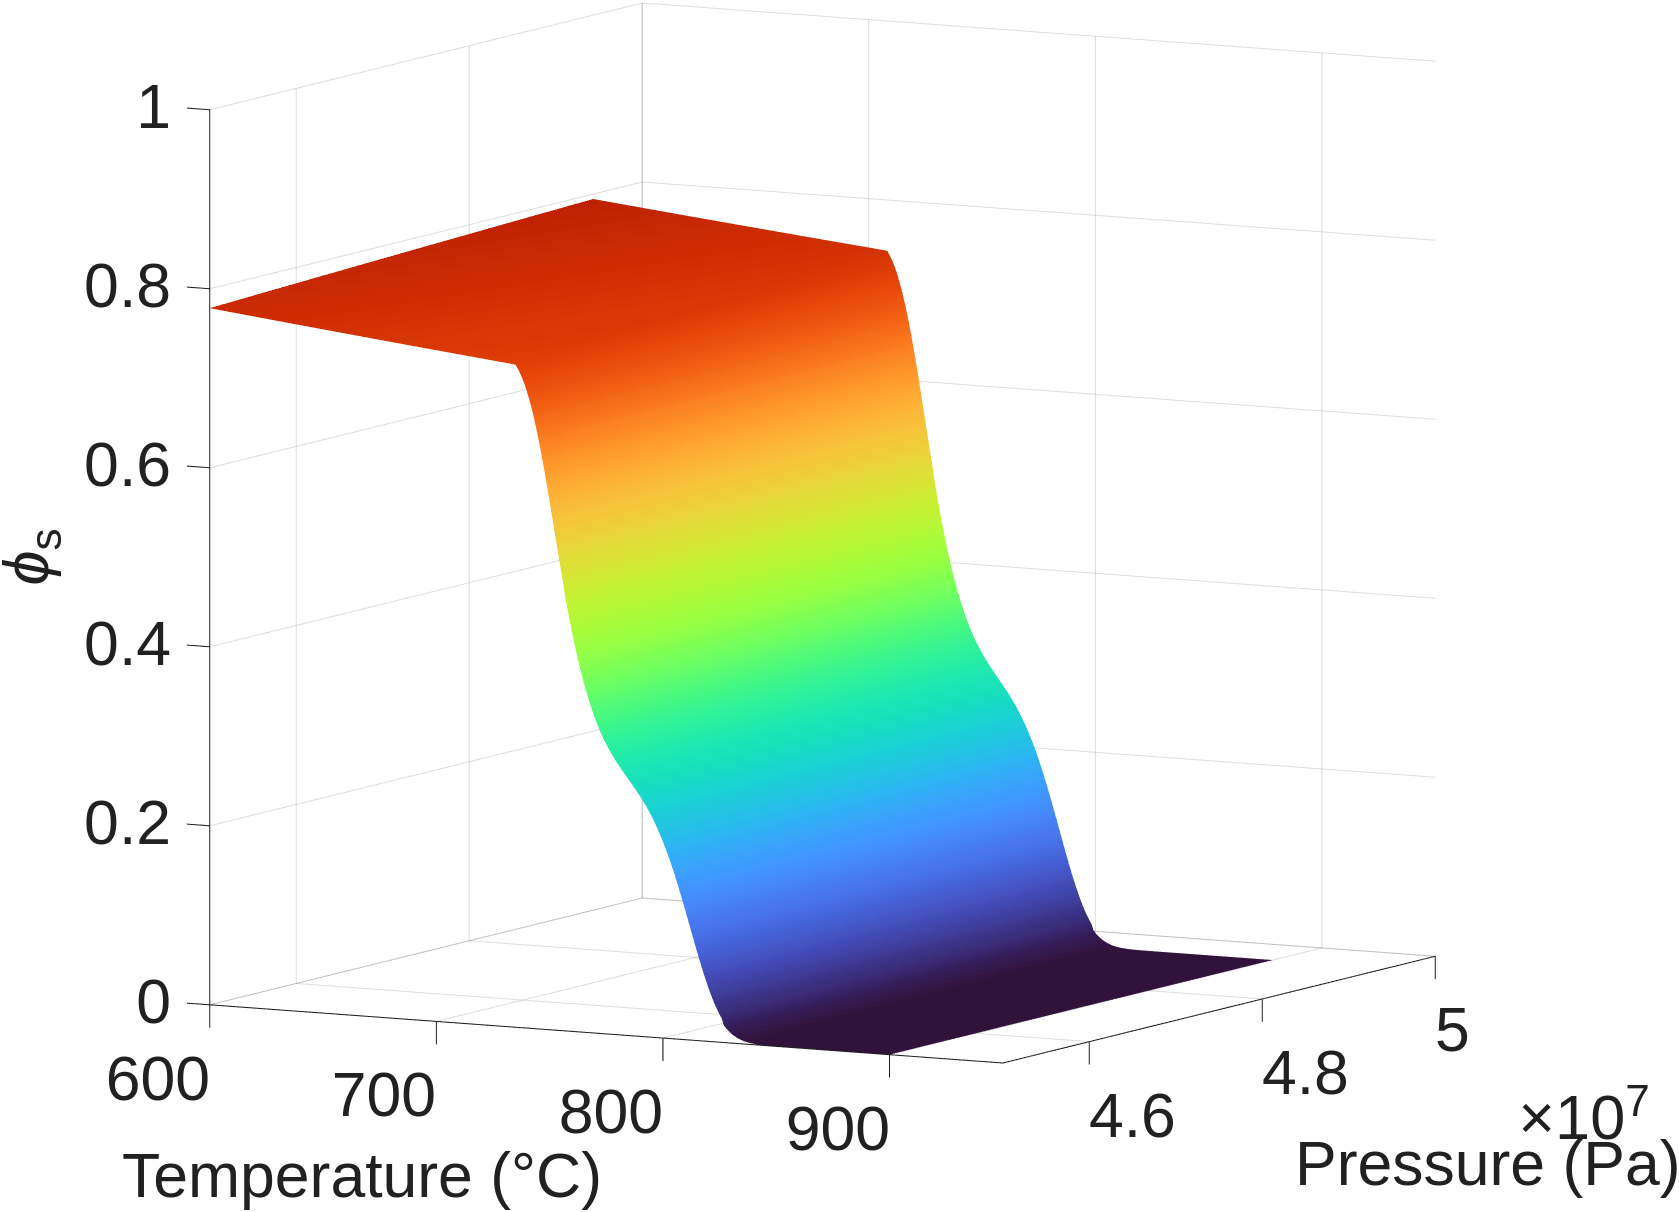
\includegraphics[width=1\linewidth]{img/chapter2/properties/vf_s/vf_s_3D.png}
	\caption{Bulk thermal conductivity modeled for 45 MPa}
	\label{fig:volume_crystals}
\end{figure}


\subsubsection{Density}
Density plays a critical role in the physical behavior and thermal evolution of magmas within the Earth's interior. It governs buoyancy-driven processes, such as magma ascent, crystal settling, magma mixing and melt segregation, which in turn influence magma chamber dynamics, volcanic eruptions, and the formation of igneous rock textures. Magma density is not constant, it varies with temperature, pressure, chemical composition (notably silica content), and volatile content (especially water and carbon dioxide). Typically, more mafic magmas are denser than felsic ones due to their higher iron and magnesium contents. As magmas cool and crystallize, the residual melt becomes more evolved and less dense, since it gets depleted in heavy elements, often leading to gravitational stratification. Additionally, the exsolution of volatiles during decompression reduces magma density, enhancing buoyancy and potentially triggering eruptions and magma mixing of deeper, more primitive, volatile rich magmas with shallower, evolved and partially degassed magmas. Overall, density controls the mechanical stability and dynamics of magma reservoirs, influencing how magmas differentiate, interact, and ultimately reach the surface.

In our model, melt density is pressure, temperature and composition dependent, obtained from the molar volume expression in \cite{lange1990}:

\begin{equation}
	V_{liq}(T,P,X_i) = \sum X_i \bigg[V_i + \frac{dV_i}{dT} (T-1673) + \frac{dV_i}{dP}(P-10^5)\bigg]
\end{equation}
\begin{equation}
	\rho = \frac{M_{liq}}{V_{liq}}
\end{equation}
where $V_{liq}$ and $M_{liq}$ are the molar volume and mass of the melt, which depend on the oxide composition. $X_{liq}$, $\frac{dV_i}{dT}$ and $ \frac{dV_i}{dP}$ the molar fraction, thermal expansion and compressibility coefficients of the $i_{th}$ oxide. The later are calculated from the data in \cite{lesher2015}.
The density of the exsolved volatile phase, which includes water and carbon dioxide, is computed with the equation of estate from SOLWCAD (\cite{papale2006}) for consistency.

\subsubsection{Heat capacity}
The heat capacity of a substance describes how much energy is required to rise the temperature of a unit of mass of said substance by one degree. It strongly governs the thermal evolution of magmatic systems by controlling how much heat magmas store and release during any process that depends upon temperature such us cooling, heating, crystallization os assimilation. Magmas with higher heat capacities, typically those with higher silica and volatile contents, can absorb more thermal energy without undergoing rapid temperature changes, leading to longer cooling times and more stable magma chambers. During crystallization, the specific heat capacity of the residual melt often increases due to the changes in composition, affecting the thermal gradient and the solidification rate.

Our model computes the specific heat capacity as the weighted average of the different oxide's heat capacities, which are obtained from \cite{lesher2015}, accounting the dissolved water:
\begin{equation}    
	cp_{melt} = \sum_{i=1}^L w_i cp_i + w_{H_2O} cp_{H_2O}
\end{equation}

Heat capacity of the gas phase is temperature dependent, obtained from a regression from classical engineering books, for both components, water and carbon dioxide:

\begin{equation}
	\begin{split}
		H_2O: &\; 1840.4 - (0.14972 \cdot T) + (9.145 \times 10^{-4} \cdot T^2) \\
		&\quad - (3.1759 \times 10^{-7} \cdot T^3) \\
		CO_2: &\; 472.27 + (1.5228 \cdot T) - (1.014 \times 10^{-3} \cdot T^2) \\
		&\quad + (2.5368 \times 10^{-7} \cdot T^3)
	\end{split}
\end{equation}

Mineral heat capacities are modeled after (burman...):

\begin{equation}
	\begin{aligned}
		cpx_{cp} &= \frac{305.41 - 1604.9\, T^{-0.5} - 7.166 \times 10^6\, T^{-2} + 9.2184 \times 10^8\, T^{-3}}{0.24855} \\[2ex]
		kfpr_{cp} &= \frac{381.37 - 1941\, T^{-0.5} - 1.20373 \times 10^7\, T^{-2} + 1.83643 \times 10^9\, T^{-3}}{0.27833} \\[2ex]
		qtz_{cp} &= \frac{80.01 - 240.3\, T^{-0.5} - 3.5467 \times 10^6\, T^{-2} + 4.9157 \times 10^8\, T^{-3}}{0.06008} \\[2ex]
		plg_{cp} &= \frac{393.64 - 2415.5\, T^{-0.5} - 7.8928 \times 10^6\, T^{-2} + 1.07064 \times 10^9\, T^{-3}}{0.26222} \\[2ex]
		mgt_{cp} &= \frac{235.90 - 1766.6\, T^{-0.5} - 1.7104 \times 10^6\, T^{-2} + 4.062 \times 10^8\, T^{-3}}{0.23153}
	\end{aligned}
\end{equation}

\begin{figure}[H]
	\centering
	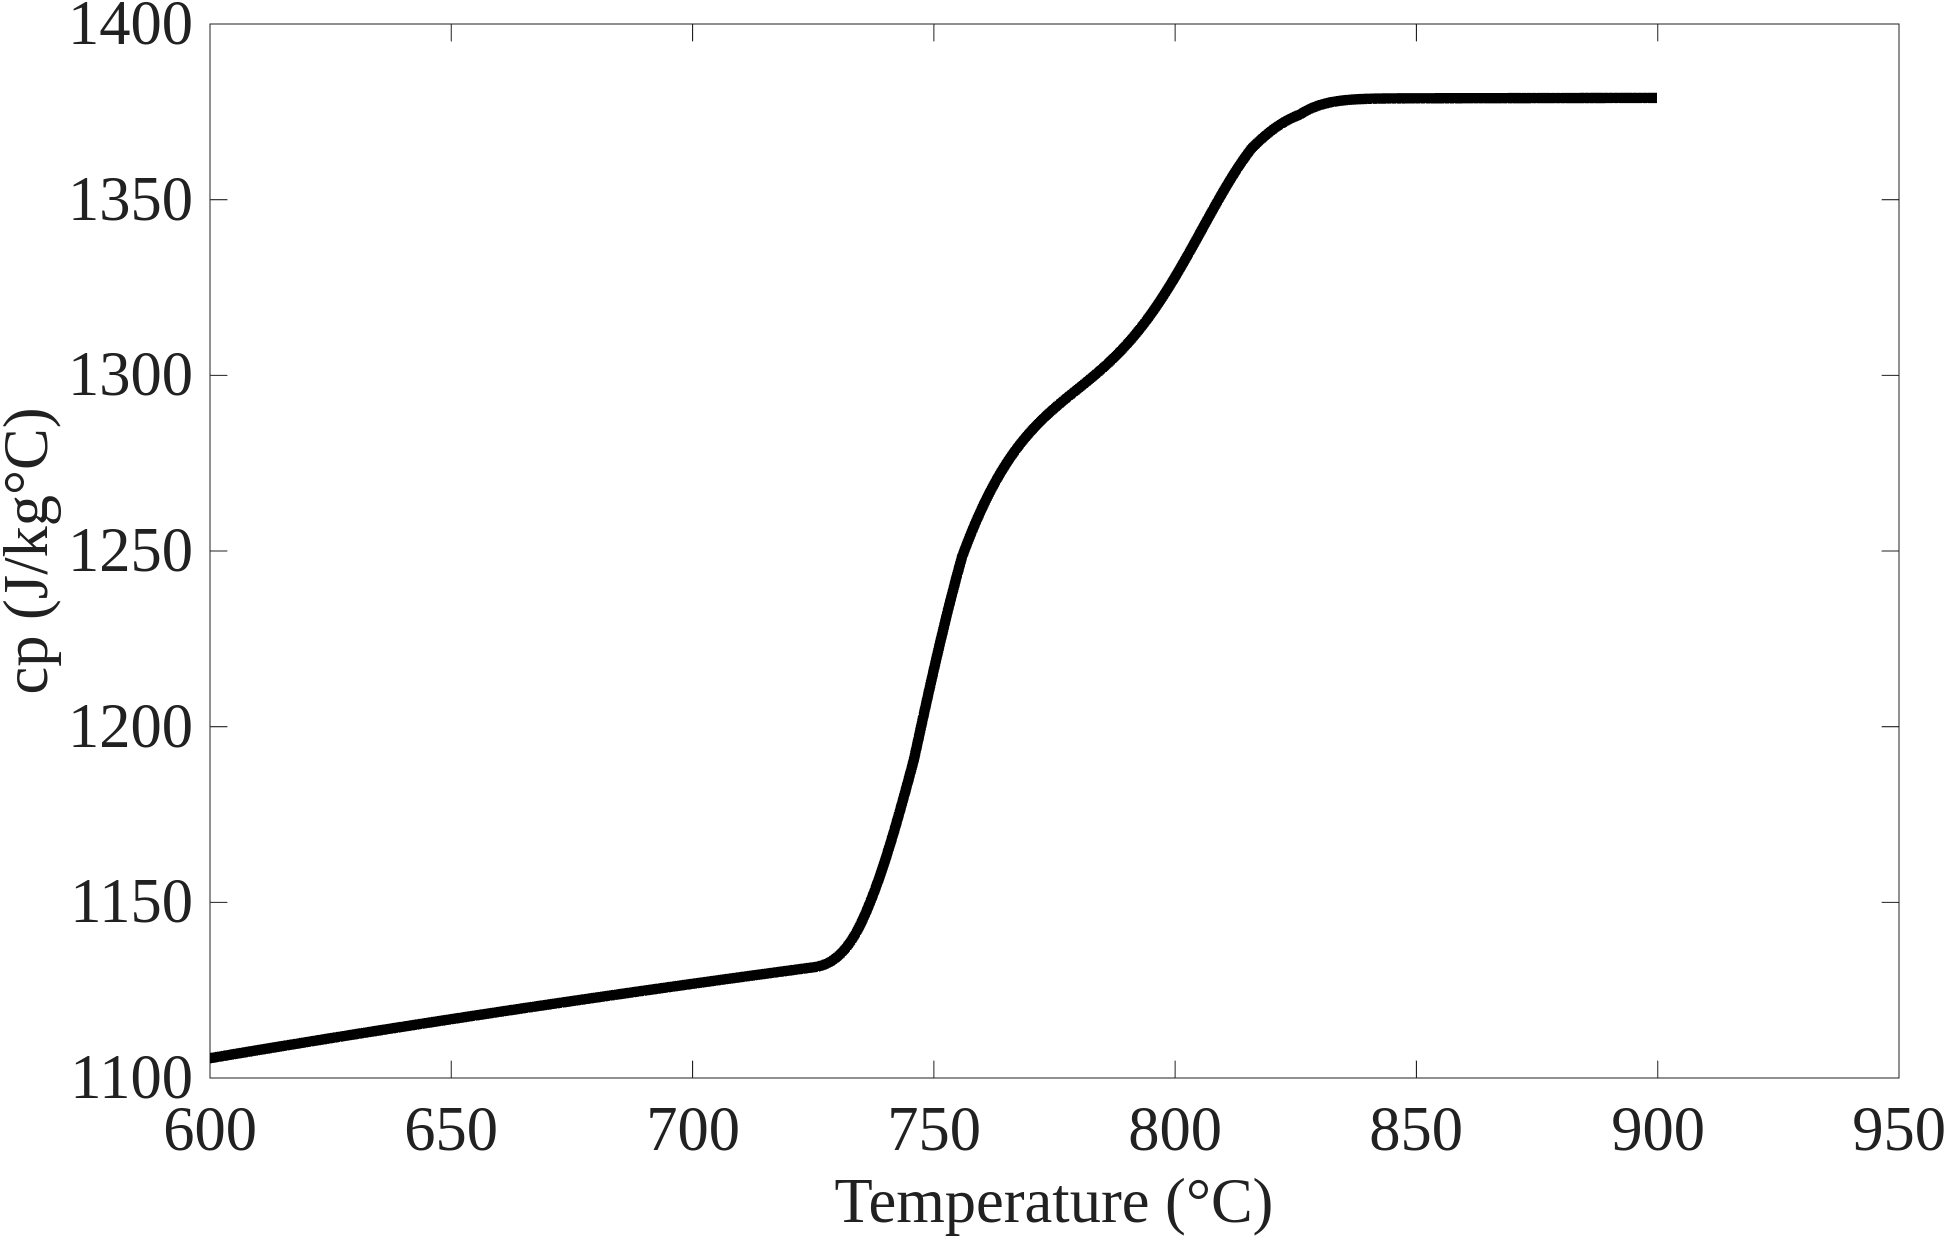
\includegraphics[width=1\linewidth]{img/chapter2/properties/heat_capacity/SMOOTHED_cp.png}
	\caption{Bulk heat capacity modeled for 45 MPa}
	\label{fig:heat_capacity}
\end{figure}

\subsubsection{Thermal conductivity}
Thermal conductivity can be defined as how efficiently heat is transmitted through any substance by molecular or lattice vibrations. It is a crucial parameter that strongly controls the rate of heat loss from magma to surrounding rocks, which influences cooling rates, crystallization times, and overall magma chamber stability. Generally, magmas have relatively low thermal conductivity compared to solid rocks, due to their disordered liquid structure and high temperatures. This low conductivity causes magmas to efficiently retain heat, contributing to the long-lived nature of magma chambers. As crystallization advances, thermal conductivity normally increases due crystals higher thermal conductivity when compared to melt. Additionally, variations in composition, crystal content, and volatile phases can cause anisotropy in thermal transport, affecting localized cooling paths and magma differentiation.

Thermal conductivity of the melt is calculated from the thermal diffusivity definition from \cite{moitra2018}
\begin{equation}
	\begin{split}
		&\alpha_L = (-0.06 + 4.57*T)\times 10^{-6}\\
		&\kappa_L = \rho_L cp_L \alpha_L\\
	\end{split}
\end{equation}
With the equation of \cite{heap2020} we calculate the thermal conductivity of combined mixture of crystals and melt.
\begin{equation}
	\begin{split}
		&\kappa_D = \frac{\kappa_L(1-\phi_c)(1-m_c) + m_c \beta_c \phi_c}{(1-\phi_c)(1-m_c) + \beta_c \phi_c}\\
		&m_c = \frac{\kappa_c}{\kappa_L} \qquad \beta_c = \frac{3(1-m_c)}{2+m_c}
	\end{split}
\end{equation}
Gas thermal conductivity is calculated from a regression of data and \cite{udoetok2013} equation for binary mixtures of gases:   
\begin{equation}
	\begin{split}
		&\kappa_G = \frac{1}{2}\bigg[\frac{\kappa_{H_2O}\kappa_{CO_2}}{\chi_{H_2O}\kappa_{H_2O} + \chi_{CO_2}\kappa_{CO_2}}\bigg] \\
		&\quad +\chi_{H_2O}\kappa_{H_2O} + \chi_{CO_2}\kappa_{CO_2}\\
		\\&\kappa_{H_2O} = 4.1771\times 10^{-3} + 2.2849\times 10^{-5}*T \\
		&\quad + 9.4663\times 10^{-8} * T^2 - 2.5778\times 10^{-11} * T^3\\
		\\&\kappa_{CO_2} = -1.0081\times 10^{-3} + 9.1422\times 10^{-5}*T \\
		&\quad - 6.4318\times 10^{-8} * T^2 - 4.31\times 10^{-11} * T^3\\
	\end{split}
\end{equation}
where $\chi_{H_2O}$ and $\chi_{CO_2}$ are the molar concentration of each component in the total gas mixture. Similarly to how it is done for the crystal and magma dense phase, we compute the bulk thermal conductivity for the dense phase plus gas phase using equation (14).

\begin{figure}[H]
	\centering
	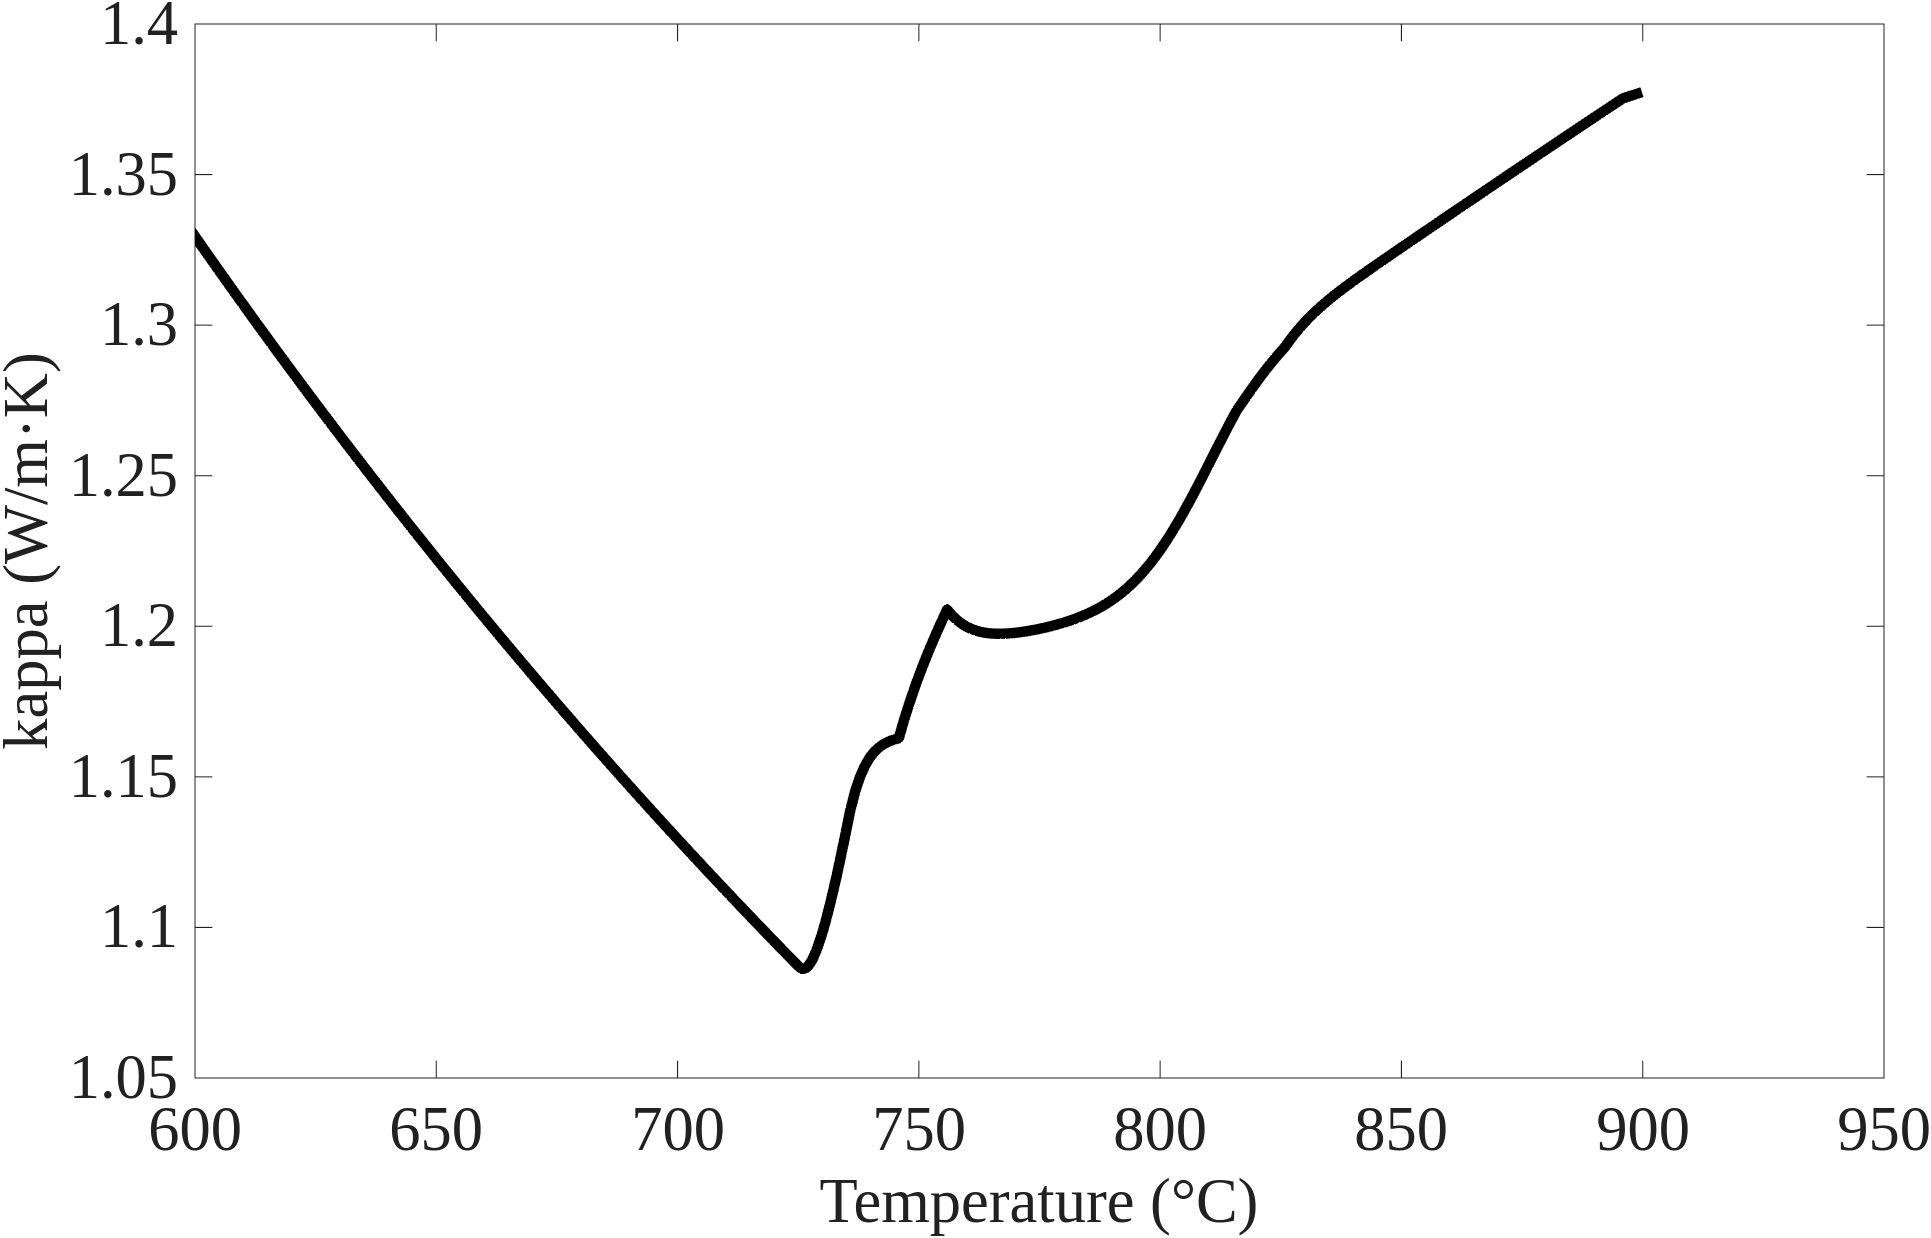
\includegraphics[width=1\linewidth]{img/chapter2/properties/kappa/SMOOTHED_kappa.png}
	\caption{Bulk thermal conductivity modeled for 45 MPa}
	\label{fig:kappa}
\end{figure}

\subsubsection{Viscosity}
Viscosity is one of the most critical physical properties of magma, which exerts major control on its flow behavior, eruption dynamics, crystallization history and many more processes. In simple words, it measures a fluid's resistance to flow and deformation. Viscosity of magmas is highly sensitive to temperature, composition and crystal and volatile content. Silica-rich magmas such as rhyolite have, generally, much higher viscosity than silica-poor, such as basalt, due to its higher state of polymerization of the silica tetrahedra within the melt. As magmas cool, viscosity increases exponentially due to the combined effect of higher polymerization and crystallization. This can strongly influence magma behavior, slowing down convection o favoring mush formation, and have a profound effect on its eruptive behavior, ranging from tranquil, effusive eruptions to violent and explosive ones with increasing viscosity, as gas bubbles struggle to coalesce and easily scape, and, as opposed, get over-pressurized. The effect of volatiles is less clear and more varied: higher dissolved volatiles content decreases magma viscosity, but exsolved bubbles can behave as rigid, non-deformable particles, hence increasing viscosity, or like deformable objects, decreasing viscosity.

In order to compute de viscosity of the system we need to account at any time and in any point in space for the combined effect of all the coexisting phase, as well as the strain rate. Due to the complexity of such system, a model that is able to able to approximate the viscosity accounting for the contribution of all these variables is yet non existent. Therefore, we tackle this issue as follows: first we compute the Newtonian viscosity according to the well known and widely used model by \cite{giordano200} and add to this viscosity the effect of crystals and strain rate applying the model by \cite{caricchi2007}, described as follows:

\begin{equation}
	\eta_r(\phi) = \frac{1 + \big(\frac{\phi}{\phi_{\text{max}}}^{\delta}\big)}
	{\bigg(1 - \alpha \, \text{erf} \bigg\{ \frac{\sqrt{\pi}}{2a} \frac{\phi}{\phi_{max}}
		\bigg[ 1 + \bigg(\frac{\phi}{\phi_{max}}\bigg)^\gamma \bigg] \bigg\}\bigg)^{\gamma \phi_{\text{max}}}}
\end{equation}

where B is the Einstein coefficient (\cite{einstein1905}) with a value of 2.5. The rest of the parameters are calculated from the following relations:

\begin{equation}
	\begin{aligned}
		\phi_{max} = 0.066499·tanh(0.913424)·log_{10}(\dot{\gamma}) + 3.850623 + 0.591806 \\
		\delta =-6.301095·tanh(0.818496·log_{10}(\dot{\gamma}) + 2.86 + 7.462405 \\
		\alpha = 0.000378·tanh(1.148101·log_{10}(\dot{\gamma}) +3.92+0.999572 \\
		\gamma = 3.987815·tanh(0.8908·log_{10}(\dot{\gamma} + 3.24 + 5.099645)        
	\end{aligned}
\end{equation}
Figure \ref{fig:viscosity}a left shows the evolution of the viscosity with temperature as if melt composition is kept change. Figure \ref{fig:viscosity}a right, on the other hand, shows the actual Newtonian evolution accounting for the change in composition due to crystallization and gas exsolution. 
To this mixture of melt and crystals we then add the contribution of gas bubbles with the also strain rate dependent model of \cite{llewellin2005}, a simplification of the model by \cite{pal2003}, which defines two regimes depending on the capillary number: with capillary numbers larger than 1, viscosity increases with the increase of the gas volume fraction, as bubbles behave rigidly. On the other hand, the second regime occurs when the capillary number is smaller than 1: bubbles are able to deform, hence, shear viscosity decreases with increasing volume fraction of gas. The capillary number can be expressed as follows:

\begin{equation}
	Ca = \frac{R\eta\dot{\gamma}}{\sigma}
\end{equation}
where R is the bubble radius, $\eta$ is the viscosity of the melt+crystals mixture, $\dot{\gamma}$ is the strain rate and $\sigma$ is the surface tension.

\cite{llewellin2005} reduce the model by \cite{pal2003} to more simple expression: 

\begin{equation}
	\begin{aligned}
		\text{If Ca < 1} \ \ \ \ \ \ \ \ \eta_r=(1-\phi_g)^{-1} \\
		\text{If Ca $\geq$ 1} \ \ \ \ \ \ \ \ \eta_r=(1-\phi_g)^{\frac{5}{3}}
	\end{aligned}
\end{equation}

where $\phi_g$ is the volume fraction of the gas phase. 
Once obtained the relative viscosity applying the effect of the gas phase, the total viscosity of the system can be easily obtained by multiplying this relative viscosity with the viscosity of the melt+crystals mixture. In addition, and for numerical stability and convergence it is necessary to fix the maximum viscosity to $10^{13}$ Pa$\cdot$s. Figure \ref{fig:viscosity}b, as opposed to figure \ref{fig:viscosity}a represents the total viscosity evolution accounting for the combined effect of melt, crystals, gas and strain rate. Figure \ref{fig:viscosity_3d}, plots the non-Newtonian viscosity for a range of strain rate and crystal volume fractions, in order to better appreciate how the combined effect translates into a strong non-linearity of the curves.


% \begin{figure}
	%     \centering
	%     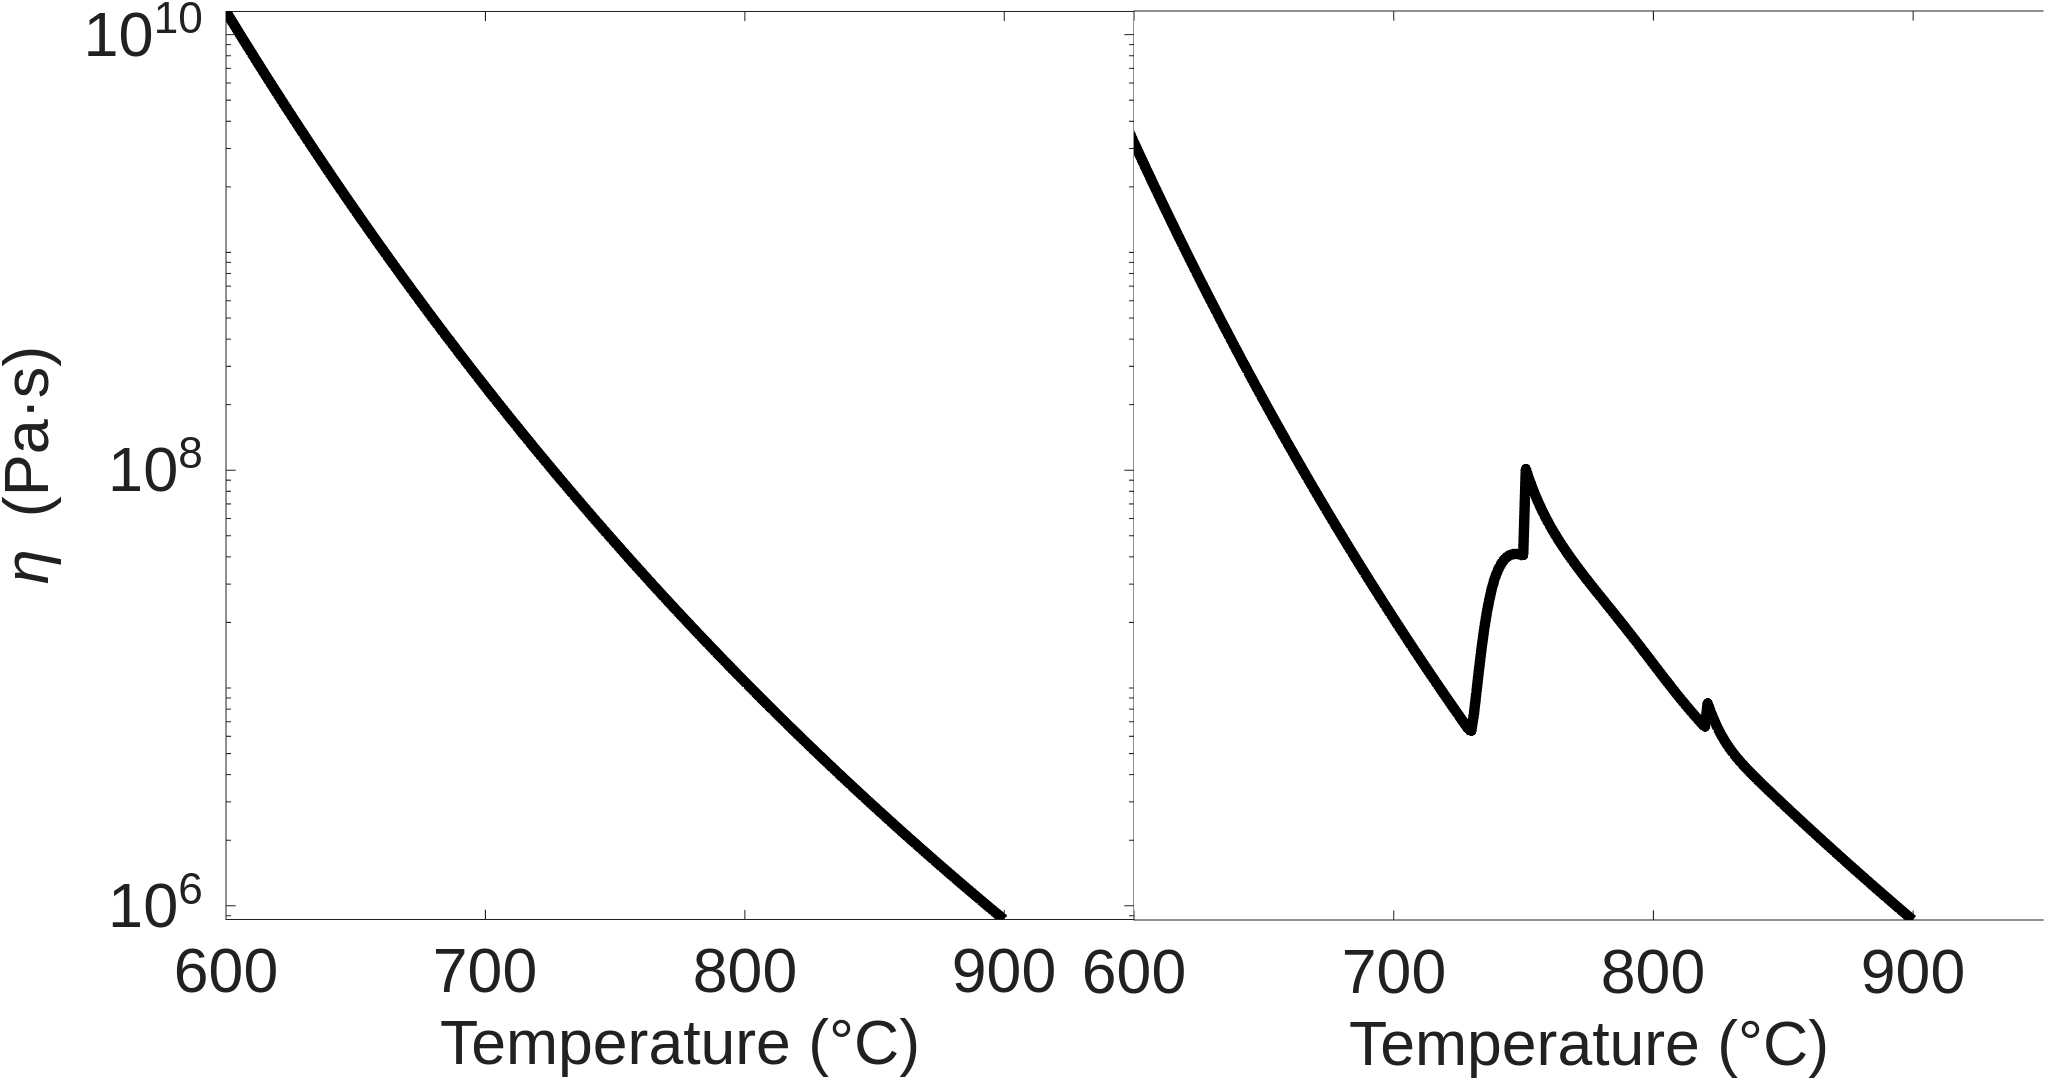
\includegraphics[width=1\linewidth]{img/chapter2/properties/viscosity/newtonian_square_30font_merged.png}
	%     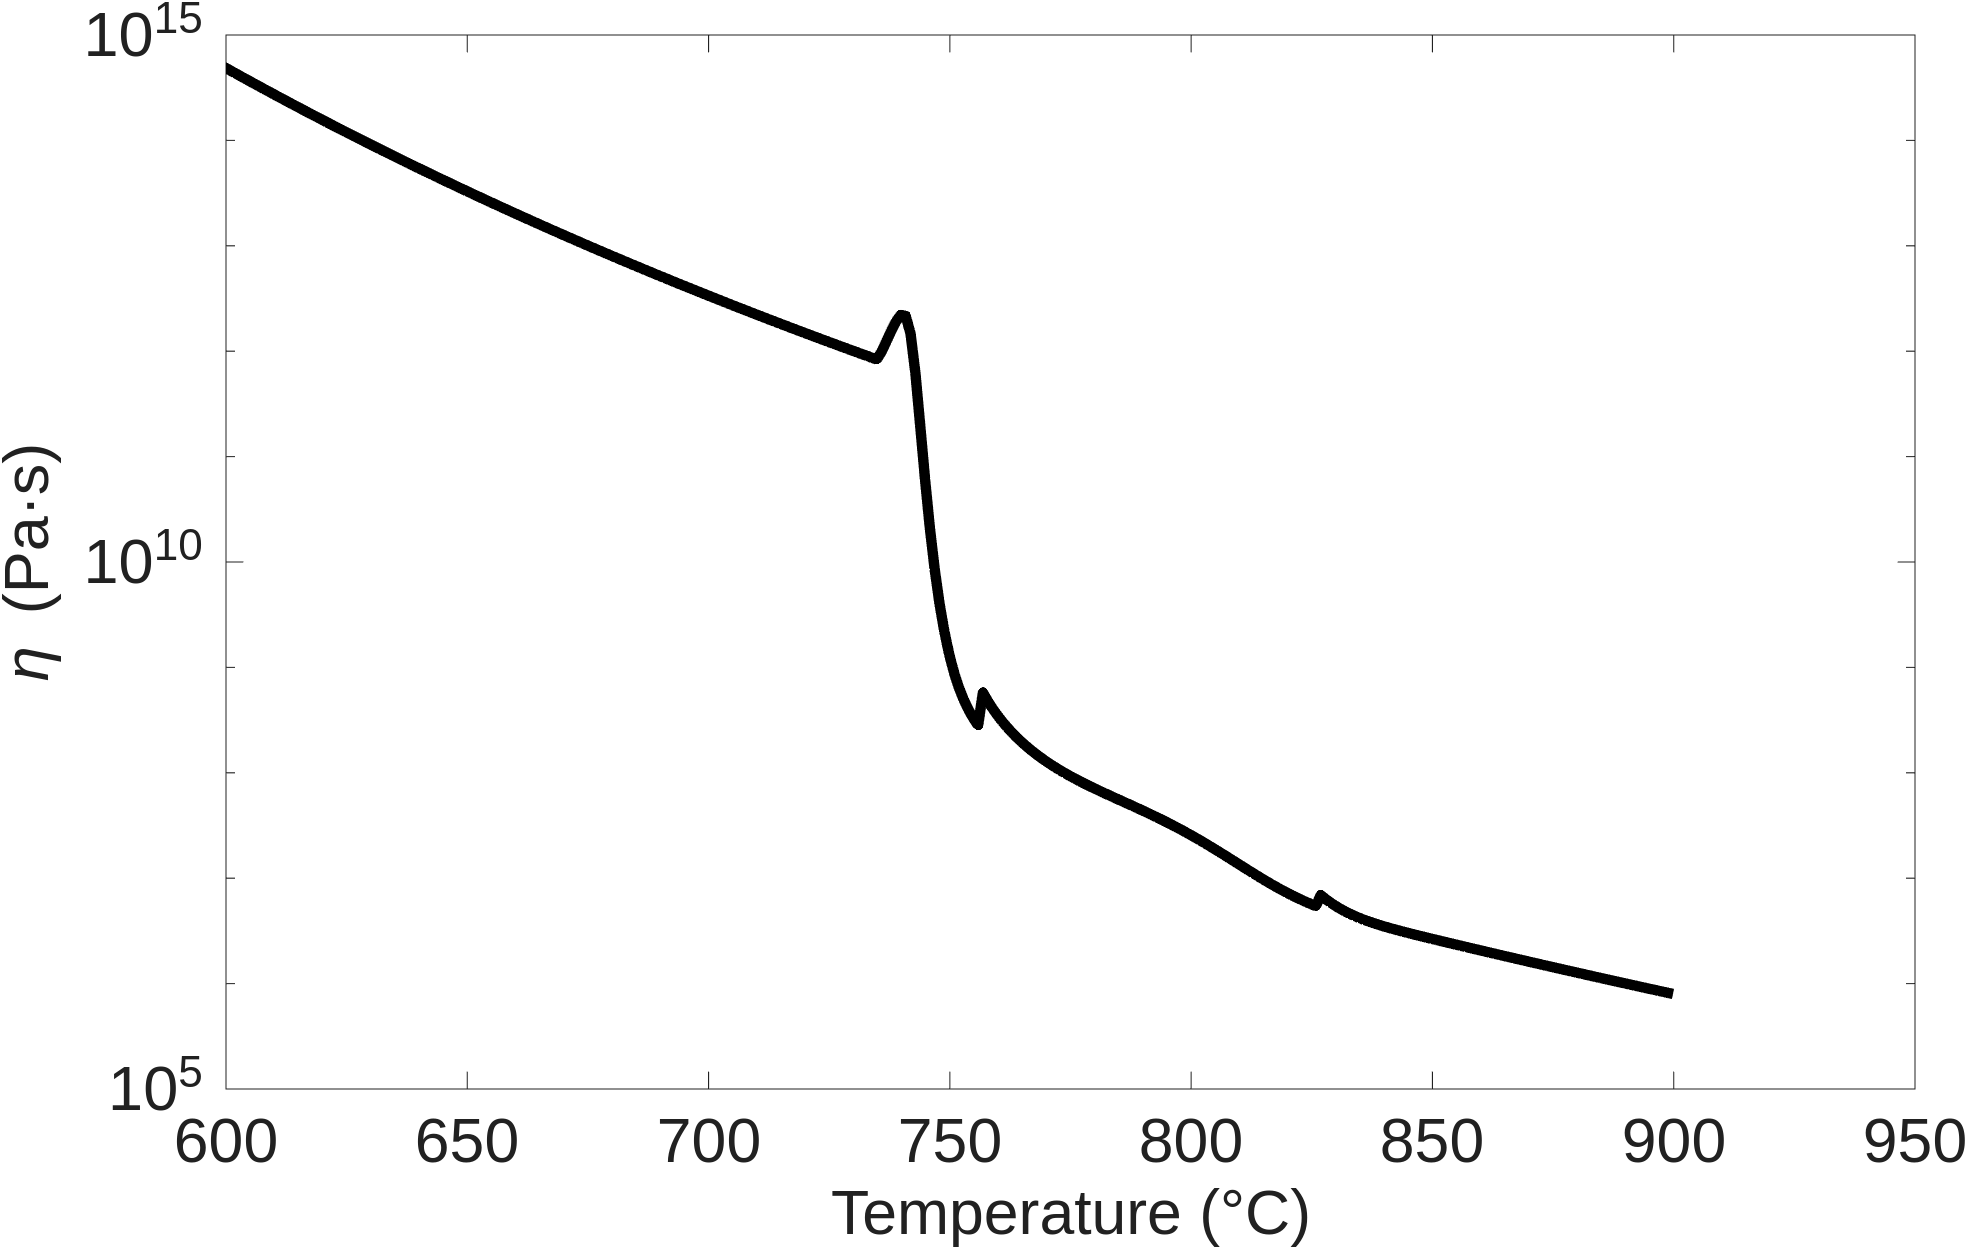
\includegraphics[width=1\linewidth]{img/chapter2/properties/viscosity/non_newt_full.png}
	%     \caption{Temperature field for the 2D convection 1c benchmark once it has reached the final steady state stage}
	%     \label{fig:enter-label}
	% \end{figure}


\begin{figure}
	\centering
	\begin{tikzpicture}
		\node[inner sep=0pt] (img1) at (0,0) {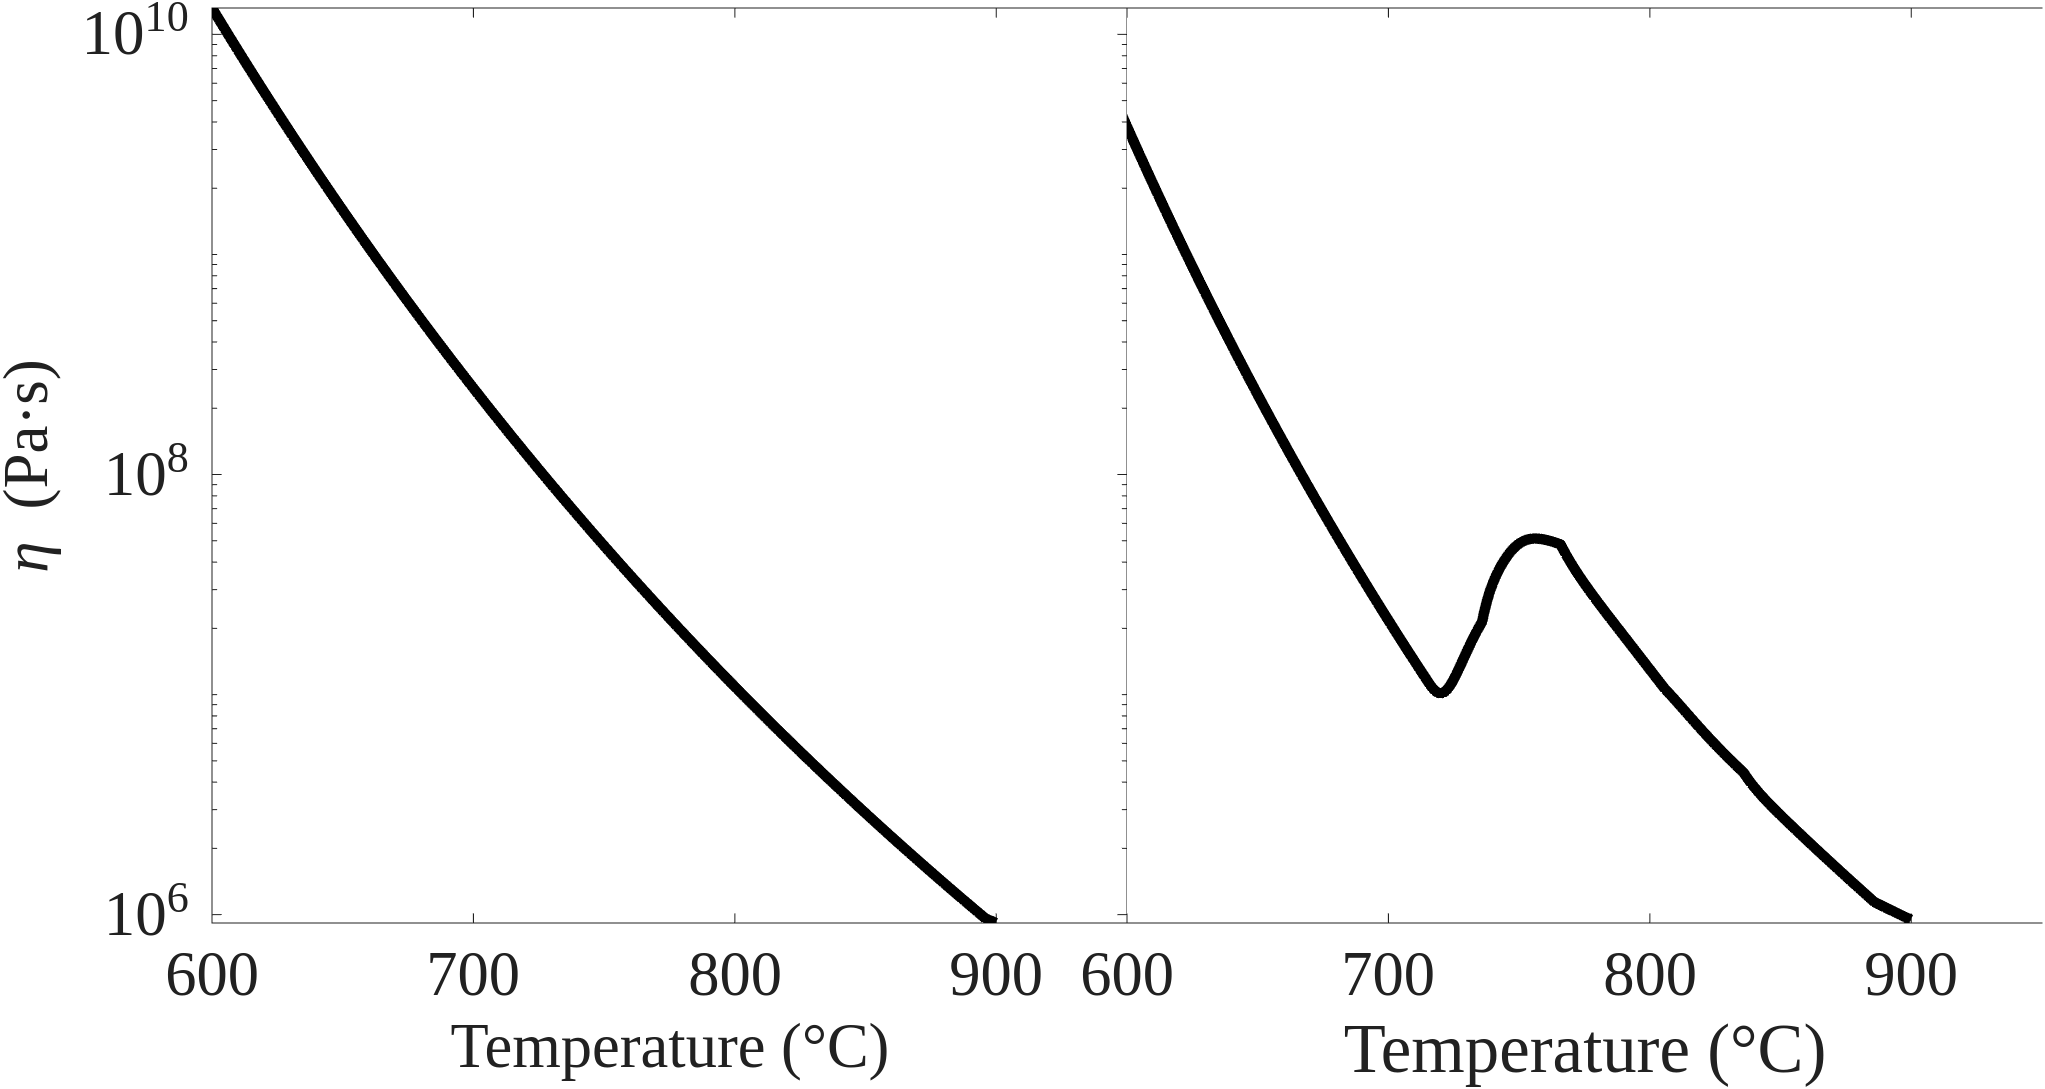
\includegraphics[width=1\linewidth]{img/chapter2/properties/viscosity/SMOOTHED_newtonian_square_30font_merged_1.png}};
		\node[anchor=north east, xshift=-8pt, yshift=-5pt] at (img1.north east) {\textbf{(a)}};
	\end{tikzpicture}
	\begin{tikzpicture}
		\node[inner sep=0pt] (img2) at (0,0) {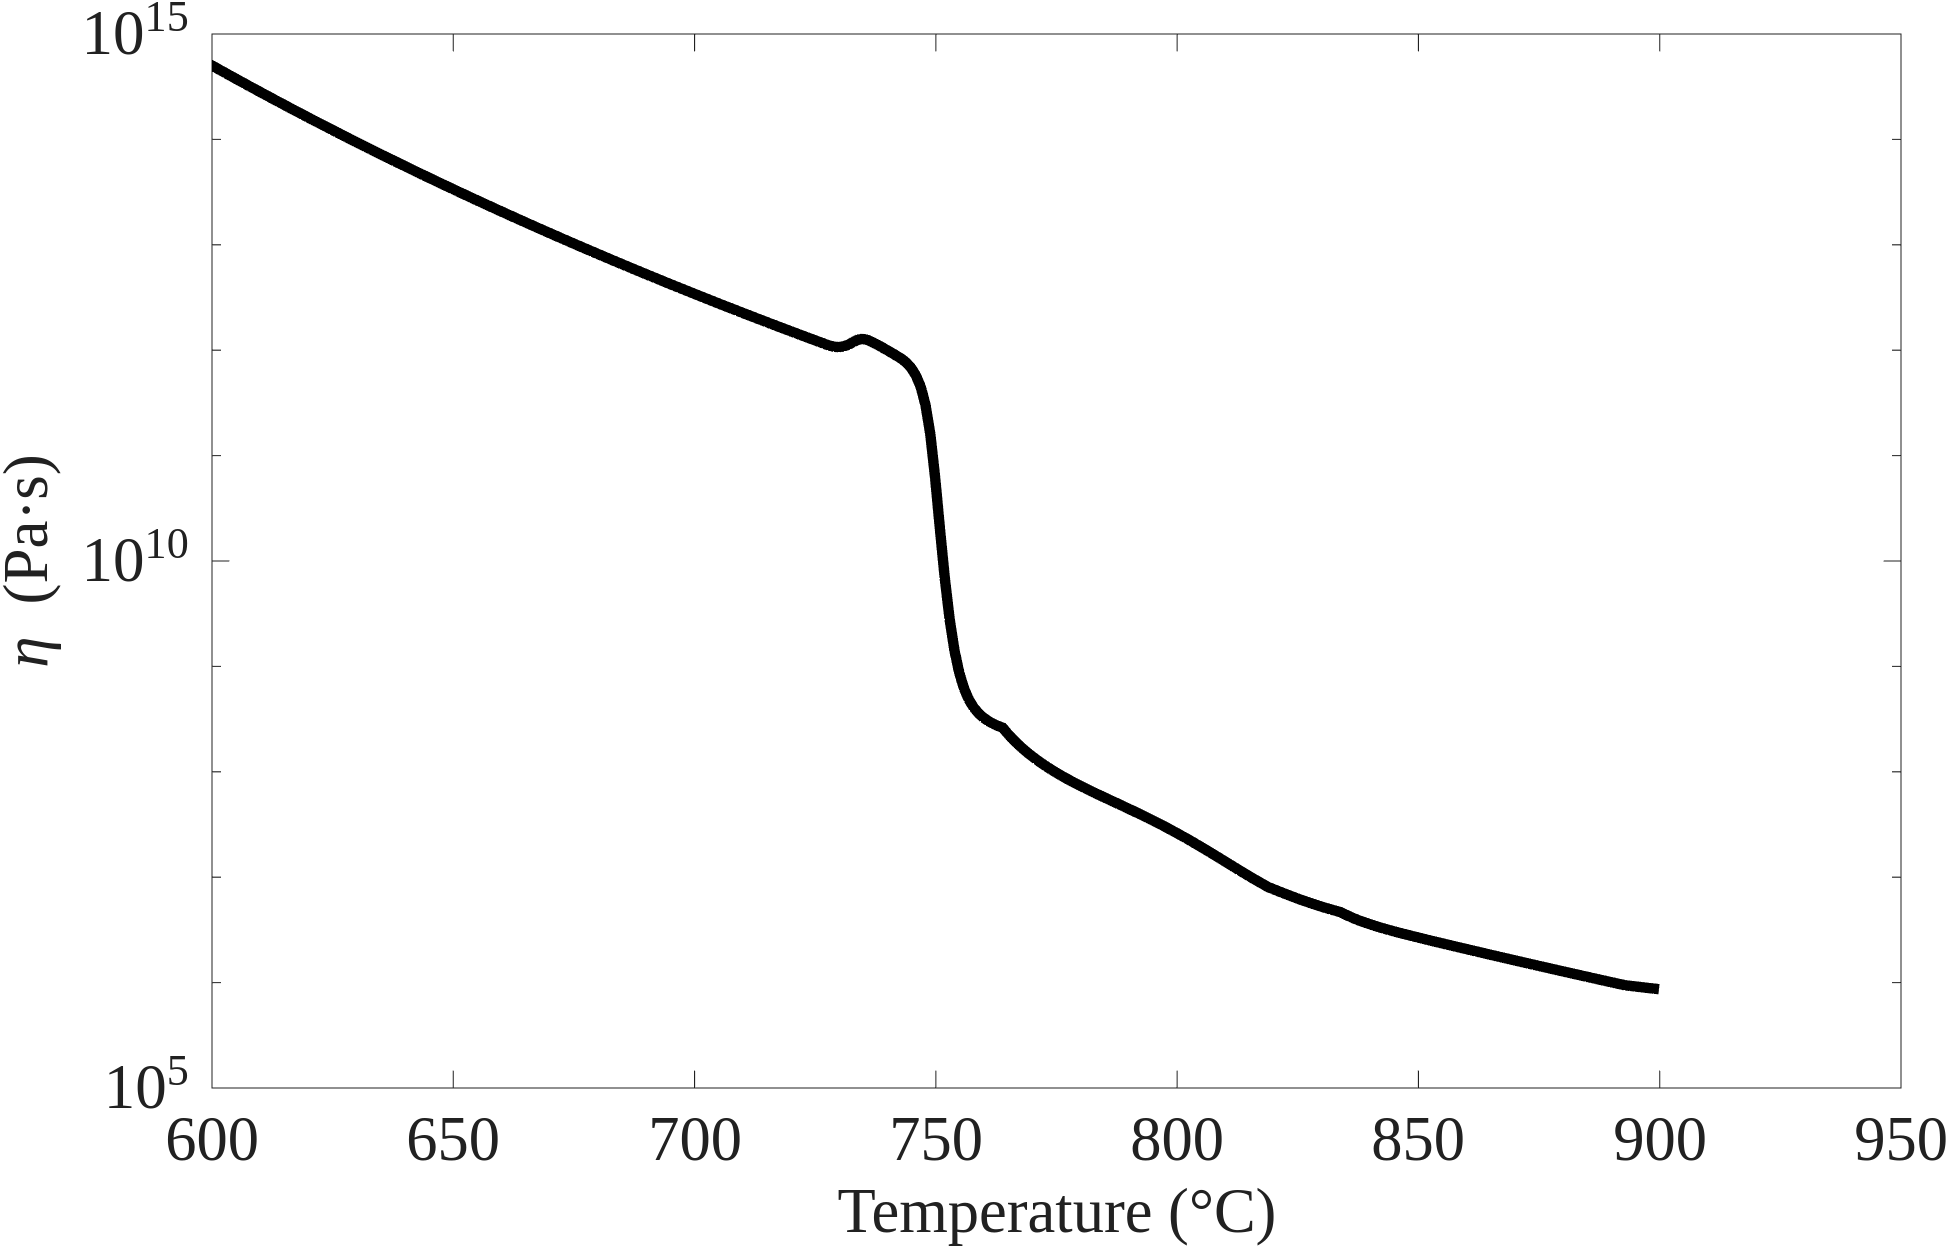
\includegraphics[width=1\linewidth]{img/chapter2/properties/viscosity/SMOOTHED_non_newt_full.png}};
		\node[anchor=north east, xshift=-8pt, yshift=-5pt] at (img2.north east) {\textbf{(b)}};
	\end{tikzpicture}
	\caption{Newtonian and non newtonian viscosity}
	\label{fig:viscosity}
\end{figure}


\begin{figure}
	\centering
	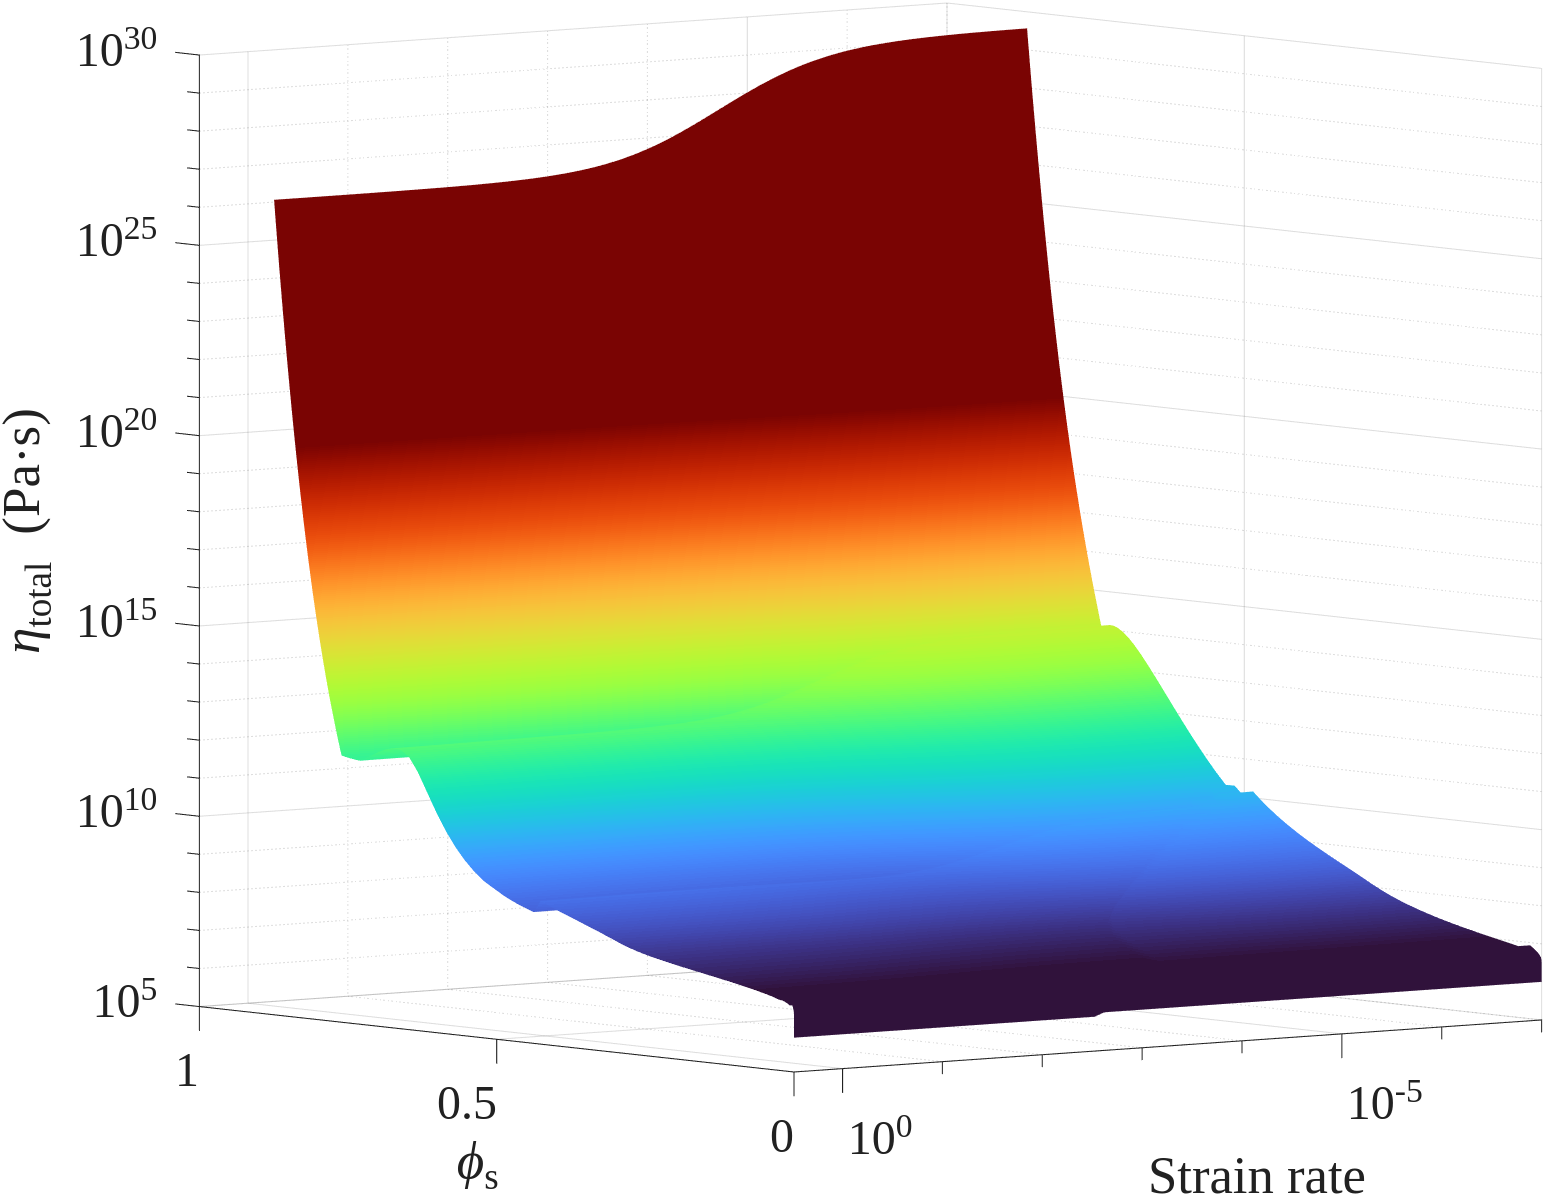
\includegraphics[width=1\linewidth]{img/chapter2/properties/viscosity/non_newt_3D_phi.png}
	\caption{Non newtoniand surface}
	\label{fig:viscosity_3d}
\end{figure}

\subsubsection{Latent heat}
Latent heat of phase change can be described as the amount of energy that is supplied of extracted from a substance in order to change its state at constant temperature and pressure. Within the context of magma kinetics, it is the heat released when a crystal is formed from the melt, or the heat absorbed by the melt when a volatile particle is exsolved. It is a fundamental magmatic process. Its influence on the energy balance of magmatic regions has being extensively studied. It partially or totally controls diverse processes that strongly affect magma emplacement, evolution and migration. \cite{depaolo1981}, \cite{huppert1988}, \cite{spera2001}, \cite{tavazzani2024} state that primitive magmatic intrusions release enough heat during crystallization to induce partial melting of the crustal rocks. \cite{anne2005}, \cite{blundy2006}, \cite{dufek2010}, \cite{namur2014}, \cite{newcombe2020}, among many others state the importance of latent heat of crystallization in buffering magma chambers against fast crystallization, suntanning deep crustal mush zones, and even influencing shallow processes like eruptions, by exerting some control over the temperature evolution during magma the ascent. It is clear then, that latent heat is not something to be overlooked, and it is of the most importance to account for its effect on our numerical simulations. 

As it is the nature itself of the latent heat of phase change, it is added to the heat transfer equation as a source term, since it can be both a source of heat, when crystallizing, or a sink of heat, when reabsorbing mineral phases or exsolving volatiles. The temperature equation is modified as follows:

\begin{equation}
	\rho c_p \left(\underbrace{\frac{\partial T}{\partial t}}_{\text{Transient term}} + \underbrace{\mathbf{v} \cdot \nabla T }_{\text{Convection term}}\right) = \underbrace{\nabla \cdot (k \nabla T)}_{\text{Conduction term}} + \underbrace{\sum_{i}^n\rho_iqL_i\phi_{i_{,t}}}_{\text{Latent heat of phase change term}}
\end{equation}

This term is described by the summation of each phase's density ($\rho_i$), its latent heat of phase change ($qL_i$) and the change on its volume fraction ($\phi_i$) with respect to time. The latent heat of phase change is computed for each phase, mineral or gas as the difference between between the heat capacity and the melt, multiplied by the increment in temperature from an standard state:

\begin{equation}
	qL_p = (cp_p-cp_L)(T-T_0)
\end{equation}

where cp$_p$ is the heat capacity of the phase, cp$_L$ is the heat capacity of the melt, T is the current temperature at the calculation point, and T$_0$ is the temperature at the standard state, that we take as 0°K. The value of $qL$ is in the order -250000 $J/Kg$ for the mineral phases and 600000 $J/Kg$ for the gas phase. As in can be expected, this term accounts for the latent heat of crystallization as well as for the heat absorbed by reabsorption or remelting of the phases.


\section{Simulation setup}
In this section, the setup for the main simulations that constitute the core of this work is explained. The simulations aim to be representative of the Krafla system, since the main objective of the work is to analyze and determine the stability conditions of the found magma, including the internal dynamics of the magma. Thus, we design a number of simulations that are representative of the Krafla system, but not only, since the results can potentially explain, hence applied to other potential shallow magmatic bodies in any other part of the world. 

Since the magma pocket, as it has being already mentioned, is yet to be constrained in size and shape by geophysical methods, the approach taken in the present work is a first order and straightforward approximation: a sill-like disk shaped magma chamber and a set of chamber sizes that are arbitrarily chosen, but representative, and of dimensions that are not larger than the resolution of usual geophysical methods, since the body (or bodies) went unnoticed under every geophysical survey that had taken place before the encounter. 

This section presents the magma domain, discussing the geometries of the simulated magmatic bodies and the different set if boundary and initial conditions such as pressure and temperature for each of the chambers. Following, the rock domain is presented in a similar way.
\subsection{Simulation domain}
\subsubsection{Magma domain}
For the magma domain, three sizes are chosen, which are referred as:\textit{small}, \textit{medium} and \textit{large}.
\textit{Small} body's long axis is 782 meters while the short axis is 156 meters. The simulated volume would be $~5*10^7 m^3$. 
Thickness and with of the \textit{medium} body are 336 meters and 1648 meters respectively, adding up to a volume of $~5*10^8 m^3$. 
Lastly, for the \textit{large} body, the dimensions are $2672x534$ meters, which would be a volume of $~2*10^9 m^3$. 

The initial temperature of the magma is set to be 900°C in all simulations, which is a consistent value with the thermometry data from \cite{elders2011} and \cite{zierenberg2013}. Initial pressure is 45 MPa for all simulations at the rooftop of the magma chamber. Pressure and volatiles content are constrained by analyzing the dissolved volatile content found in the glass cuttings (1.77 wt\% of $H_2O$ and 85 ppm $CO_2$ according to \cite{elders2014}). Any pair of dissolved $H_2O$ and $CO_2$ provides only one entrapment pressure and composition of the gas phase for any given redox conditions, which means that, knowing the dissolved quantities and the redox conditions, the gas composition and entrapment pressure can be calculated utilizing SOLWCAD. This is better shown in figure XX, where we can see that for the dissolved volatiles content, the computations throw an entrapment pressure of 45.4 MPa for which the amount of $CO_2$ in the gas phase should be 58.9 wt\%. However, this computations deliver the pressure and the gas phase composition, but there are infinite pairs of total (dissolved and exsolved) volatiles for the set redox conditions which lay in a straight line (as in figure XX). The minimum volatiles content is the one found in the glass cuttings, that would mean there are no exsolved volatiles. However, in order to be as consistent as possible with the general reality, the base total volatiles content in the base simulations is set to be 2 wt\% of $H_2O$ and 0.352 wt\% of $CO_2$. This pair means that the exsolved volatiles phase should be around 9.5\% volume for the calculated pressure. 

Initial velocity inside the domain is 0 m/s. No slip conditions are applied to the boundary. Boundary temperature is not computed in the magma domain, but instead is passed as a Dirichlet boundary condition from the solution of the host rock temperature.


\begin{table}[H]
	\resizebox{\columnwidth}{!}{%
		\begin{tabular}{|c|c|c|c|c|c|c|}
			\hline
			& long axis (m) & short axis (m) & vol (m$^3$) & $T_{\mathrm{init}}$ (°C) & $P_{\mathrm{init}}$ (MPa) & $H_2O^{\mathrm{tot}}$, $CO_2^{\mathrm{tot}}$ (wt\%) \\
			\hline
			Small & 782 & 156 & $\sim 5 \times 10^{7}$ & 900 & 45 & 2, 0.352 \\
			\hline
			Medium & 1648 & 336 & $\sim 5 \times 10^{8}$ & 900 & 45 / 50 & (2 ; 0.352) / (1.77 ; 85 ppm) / (2.5 ; 1.105) \\
			\hline
			Large & 2672 & 156 & $\sim 2 \times 10^{9}$ & 900 & 45 & 2, 0.352 \\
			\hline
		\end{tabular}%
	}
	\caption{This table summarizes the set of conditions for the different simulations carried for the three different sizes. Along the work, a base simulation is one with 45 MPa initial pressure and 2 wt\% $H_2O$ and 0.352 wt\% $CO_2$.}
	\label{tab:simulations_setup}
\end{table}

\subsubsection{Rock domain}
The rock domain is quite simpler. It is set to be a 4 km by 4 km squared box surrounding the magma body. A geothermal of 0.16°C/m from the surface. This ensures that the temperature at the 2070 meters is 350°C, which is in accordance to the temperature registered by the IDDP-1 temperature log. A steeper geothermal gradient (18.3°C/m) is imposed in the last 30 meters around the magma pocket, since temperature needs to rise from 350°C up to the magmatic temperature.

For the shake of simplicity, the properties of the rock domain are set as fixed. Density is set to 

The temperature at the surface boundary is fixed to 0°C, while the rest of the domain is free to evolve.
The overall setup can be better seen in figure \ref{fig:ic_bc}. Top image represents the domains of the three different bodies, while the bottom image a zoomed version of one of the domains with the a schematic representation of the initial and coupling conditions for the base simulations. 

\begin{figure}
	\centering
	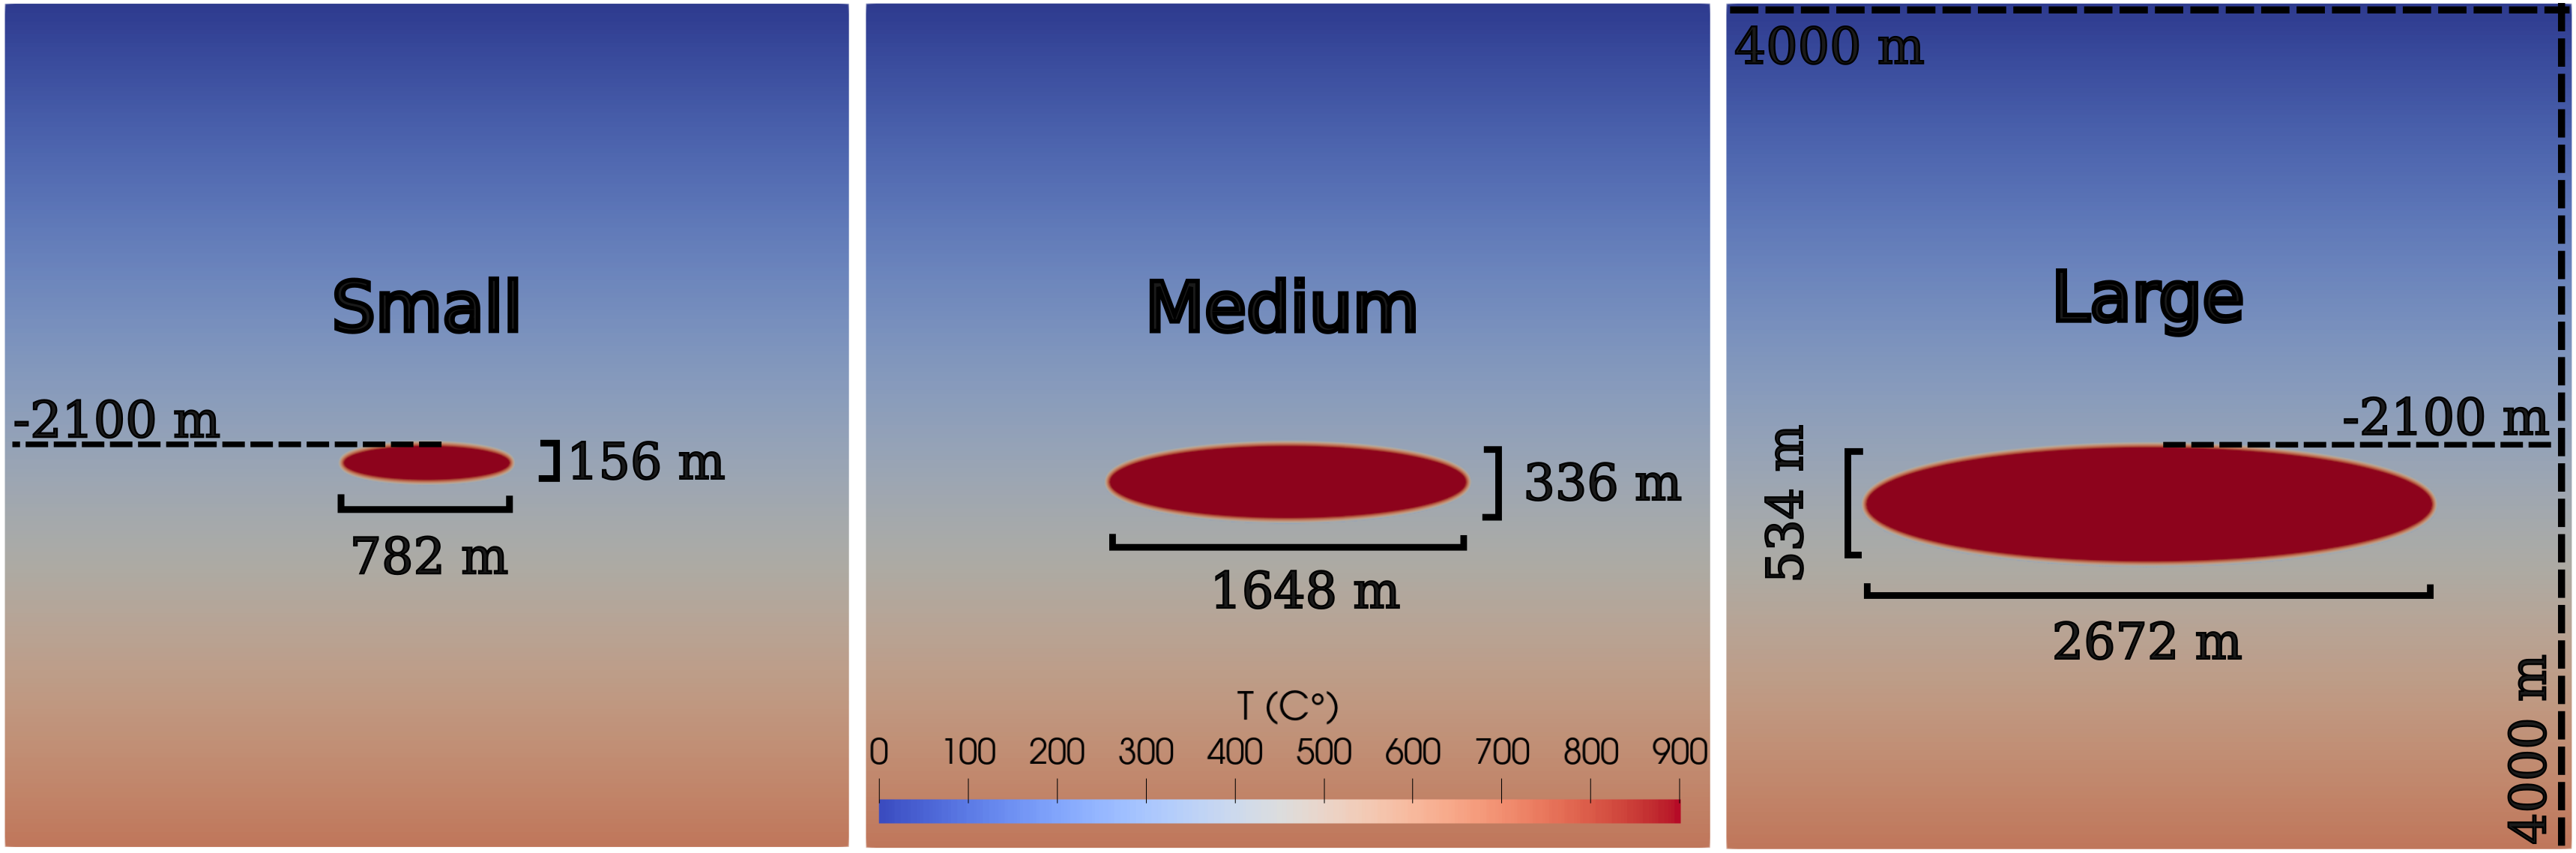
\includegraphics[width=1\linewidth]{img/chapter2/sim_setup/ic_cut.png}
	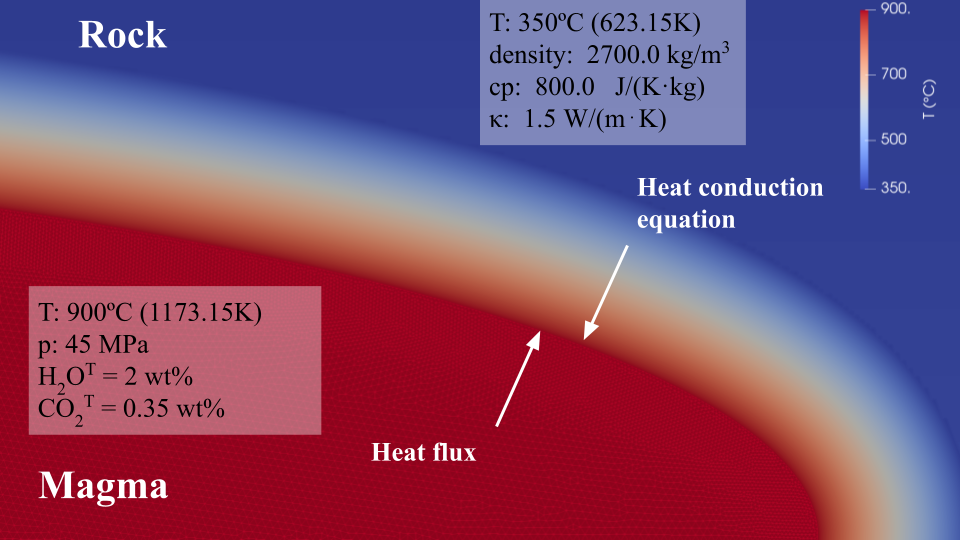
\includegraphics[width=1\linewidth]{img/chapter2/sim_setup/setup.png}
	\caption{Temperature field for the 2D convection 1c benchmark once it has reached the final steady state stage}
	\label{fig:ic_bc}
\end{figure}

